\documentclass[a4paper,12pt,twoside]{memoir}

% Castellano
\usepackage[spanish,es-tabla]{babel}
\selectlanguage{spanish}
\usepackage[utf8]{inputenc}
\usepackage[T1]{fontenc}
\usepackage{lmodern} % scalable font
\usepackage{microtype}
\usepackage{placeins}

\RequirePackage{booktabs}
\RequirePackage[table]{xcolor}
\RequirePackage{xtab}
\RequirePackage{multirow}

% Links
\usepackage[colorlinks]{hyperref}
\hypersetup{
	allcolors = {red}
}

% Ecuaciones
\usepackage{amsmath}

% Rutas de fichero / paquete
\newcommand{\ruta}[1]{{\sffamily #1}}

% Párrafos
\nonzeroparskip


% Imagenes
\usepackage{graphicx}
\newcommand{\imagen}[2]{
	\begin{figure}[!h]
		\centering
		\includegraphics[width=0.9\textwidth]{#1}
		\caption{#2}\label{fig:#1}
	\end{figure}
	\FloatBarrier
}

\newcommand{\imagenflotante}[2]{
	\begin{figure}%[!h]
		\centering
		\includegraphics[width=0.9\textwidth]{#1}
		\caption{#2}\label{fig:#1}
	\end{figure}
}

\usepackage{eurosym}

\widowpenalty10000
\clubpenalty10000

\usepackage{dirtree}

\newcommand{\hubu}{\hline \rule{0pt}{2.7ex}}

% El comando \figura nos permite insertar figuras comodamente, y utilizando
% siempre el mismo formato. Los parametros son:
% 1 -> Porcentaje del ancho de página que ocupará la figura (de 0 a 1)
% 2 --> Fichero de la imagen
% 3 --> Texto a pie de imagen
% 4 --> Etiqueta (label) para referencias
% 5 --> Opciones que queramos pasarle al \includegraphics
% 6 --> Opciones de posicionamiento a pasarle a \begin{figure}
\newcommand{\figuraConPosicion}[6]{%
  \setlength{\anchoFloat}{#1\textwidth}%
  \addtolength{\anchoFloat}{-4\fboxsep}%
  \setlength{\anchoFigura}{\anchoFloat}%
  \begin{figure}[#6]
    \begin{center}%
      \Ovalbox{%
        \begin{minipage}{\anchoFloat}%
          \begin{center}%
            \includegraphics[width=\anchoFigura,#5]{#2}%
            \caption{#3}%
            \label{#4}%
          \end{center}%
        \end{minipage}
      }%
    \end{center}%
  \end{figure}%
}

%
% Comando para incluir imágenes en formato apaisado (sin marco).
\newcommand{\figuraApaisadaSinMarco}[5]{%
  \begin{figure}%
    \begin{center}%
    \includegraphics[angle=90,height=#1\textheight,#5]{#2}%
    \caption{#3}%
    \label{#4}%
    \end{center}%
  \end{figure}%
}
% Para las tablas
\newcommand{\otoprule}{\midrule [\heavyrulewidth]}
%
% Nuevo comando para tablas pequeñas (menos de una página).
\newcommand{\tablaSmall}[5]{%
 \begin{table}
  \begin{center}
   \rowcolors {2}{gray!35}{}
   \begin{tabular}{#2}
    \toprule
    #4
    \otoprule
    #5
    \bottomrule
   \end{tabular}
   \caption{#1}
   \label{tabla:#3}
  \end{center}
 \end{table}
}

%
%Para el float H de tablaSmallSinColores
\usepackage{float}

%
% Nuevo comando para tablas pequeñas (menos de una página).
\newcommand{\tablaSmallSinColores}[5]{%
 \begin{table}[h]
  \begin{center}
   \begin{tabular}{#2}
    \toprule
    #4
    \otoprule
    #5
    \bottomrule
   \end{tabular}
   \caption{#1}
   \label{tabla:#3}
  \end{center}
 \end{table}
}

\newcommand{\tablaApaisadaSmall}[5]{%
\begin{landscape}
  \begin{table}
   \begin{center}
    \rowcolors {2}{gray!35}{}
    \begin{tabular}{#2}
     \toprule
     #4
     \otoprule
     #5
     \bottomrule
    \end{tabular}
    \caption{#1}
    \label{tabla:#3}
   \end{center}
  \end{table}
\end{landscape}
}

%
% Nuevo comando para tablas grandes con cabecera y filas alternas coloreadas en gris.
\newcommand{\tabla}[6]{%
  \begin{center}
    \tablefirsthead{
      \toprule
      #5
      \otoprule
    }
    \tablehead{
      \multicolumn{#3}{l}{\small\sl continúa desde la página anterior}\\
      \toprule
      #5
      \otoprule
    }
    \tabletail{
      \hline
      \multicolumn{#3}{r}{\small\sl continúa en la página siguiente}\\
    }
    \tablelasttail{
      \hline
    }
    \bottomcaption{#1}
    \rowcolors {2}{gray!35}{}
    \begin{xtabular}{#2}
      #6
      \bottomrule
    \end{xtabular}
    \label{tabla:#4}
  \end{center}
}

%
% Nuevo comando para tablas grandes con cabecera.
\newcommand{\tablaSinColores}[6]{%
  \begin{center}
    \tablefirsthead{
      \toprule
      #5
      \otoprule
    }
    \tablehead{
      \multicolumn{#3}{l}{\small\sl continúa desde la página anterior}\\
      \toprule
      #5
      \otoprule
    }
    \tabletail{
      \hline
      \multicolumn{#3}{r}{\small\sl continúa en la página siguiente}\\
    }
    \tablelasttail{
      \hline
    }
    \bottomcaption{#1}
    \begin{xtabular}{#2}
      #6
      \bottomrule
    \end{xtabular}
    \label{tabla:#4}
  \end{center}
}

%
% Nuevo comando para tablas grandes sin cabecera.
\newcommand{\tablaSinCabecera}[5]{%
  \begin{center}
    \tablefirsthead{
      \toprule
    }
    \tablehead{
      \multicolumn{#3}{l}{\small\sl continúa desde la página anterior}\\
      \hline
    }
    \tabletail{
      \hline
      \multicolumn{#3}{r}{\small\sl continúa en la página siguiente}\\
    }
    \tablelasttail{
      \hline
    }
    \bottomcaption{#1}
  \begin{xtabular}{#2}
    #5
   \bottomrule
  \end{xtabular}
  \label{tabla:#4}
  \end{center}
}



\definecolor{cgoLight}{HTML}{EEEEEE}
\definecolor{cgoExtralight}{HTML}{FFFFFF}

%
% Nuevo comando para tablas grandes sin cabecera.
\newcommand{\tablaSinCabeceraConBandas}[5]{%
  \begin{center}
    \tablefirsthead{
      \toprule
    }
    \tablehead{
      \multicolumn{#3}{l}{\small\sl continúa desde la página anterior}\\
      \hline
    }
    \tabletail{
      \hline
      \multicolumn{#3}{r}{\small\sl continúa en la página siguiente}\\
    }
    \tablelasttail{
      \hline
    }
    \bottomcaption{#1}
    \rowcolors[]{1}{cgoExtralight}{cgoLight}

  \begin{xtabular}{#2}
    #5
   \bottomrule
  \end{xtabular}
  \label{tabla:#4}
  \end{center}
}




\graphicspath{ {./img/} }

% Capítulos
\chapterstyle{bianchi}
\newcommand{\capitulo}[2]{
	\setcounter{chapter}{#1}
	\setcounter{section}{0}
	\chapter*{#2}
	\addcontentsline{toc}{chapter}{#2}
	\markboth{#2}{#2}
}

% Apéndices
\renewcommand{\appendixname}{Apéndice}
\renewcommand*\cftappendixname{\appendixname}

\newcommand{\apendice}[1]{
	%\renewcommand{\thechapter}{A}
	\chapter{#1}
}

\renewcommand*\cftappendixname{\appendixname\ }

% Formato de portada
\makeatletter
\usepackage{xcolor}
\newcommand{\tutor}[1]{\def\@tutor{#1}}
\newcommand{\course}[1]{\def\@course{#1}}
\definecolor{cpardoBox}{HTML}{E6E6FF}
\def\maketitle{
  \null
  \thispagestyle{empty}
  % Cabecera ----------------
\noindent
\includegraphics[width=\textwidth]{cabecera}\vspace{1cm}%
  \vfill
  % Título proyecto y escudo informática ----------------
  \colorbox{cpardoBox}{%
    \begin{minipage}{.8\textwidth}
      \vspace{.5cm}\Large
      \begin{center}
      \textbf{TFG del Grado en Ingeniería Informática}\vspace{.6cm}\\
      \textbf{\LARGE\@title{}}
      \end{center}
      \vspace{.2cm}
    \end{minipage}

  }%
  \hfill\begin{minipage}{.20\textwidth}
    
\includegraphics[width=\textwidth]{escudoInfor}
  \end{minipage}
  \vfill
  % Datos de alumno, curso y tutores ------------------
  \begin{center}%
  {%
    \noindent\LARGE
    Presentado por \@author{}\\ 
    en Universidad de Burgos --- \@date{}\\
    Tutores: \@tutor{}\\
  }%
  \end{center}%
  \null
  \cleardoublepage
  }
\makeatother


% Datos de portada
\title{AVC\\ Asistente Virtual para la Comunicación\\Anexos}
\author{José Miguel Ramírez Sanz}
\tutor{Dr. José Francisco Díez Pastor y Dr. César Represa Pérez}
\date{\today}

\begin{document}

\maketitle



\cleardoublepage



%%%%%%%%%%%%%%%%%%%%%%%%%%%%%%%%%%%%%%%%%%%%%%%%%%%%%%%%%%%%%%%%%%%%%%%%%%%%%%%%%%%%%%%%



\frontmatter


\clearpage

% Indices
\tableofcontents

\clearpage

\listoffigures

\clearpage

\listoftables

\clearpage

\mainmatter

\appendix

\apendice{Plan de Proyecto Software}

\section{Introducción}
La planificación de un proyecto es esencial para su éxito, ya que nos permite ver cuales van a ser las necesidades, los impedimentos y otra serie de eventos o circunstancias relevantes en el desarrollo de este. La planificación de un proyecto software tiene diversas partes que tratan temas como la planificación temporal o el uso de licencias.

La planificación de este proyecto se ha divido en dos secciones:
\begin{itemize}
	\item \textbf{Planificación temporal:} sección donde se puede ver la distribución temporal del proyecto, dividido en \textit{sprints}. Cada \textit{sprint} está formado por una serie de tareas relacionadas con una estimación individual de tiempo. 
	\item \textbf{Estudio de viabilidad:} sección orientada a la viabilidad del proyecto, es decir, que tan favorable es su realización en aspectos económicos y legales.
	\begin{itemize}
		\item \textbf{Viabilidad económica:} en esta subsección comentaré los gastos que ha tenido el desarrollo del proyecto.
		\item \textbf{Viabilidad legal:} subsección en la que expondré las distintas licencias de las librerías que han sido necesarias para el desarrollo del proyecto y la licencia final del producto.
	\end{itemize}
\end{itemize}

En este proyecto he seguido, además, la metodología \textit{SCRUM} gracias a la \textit{GitHub} junto con \textit{ZenHub}, pudiendo así hacer una planificación correcta y desarrollo incremental.
\section{Planificación temporal}
En esta sección voy a comentar el desarrollo temporal del proyecto divido en distintos \textit{sprints}, por cada uno de ellos voy a comentar:
\begin{itemize}
	\item Fecha de inicio y de cierre del \textit{sprint}.
	\item Pequeña descripción de lo que se pretendía hacer en el \textit{sprint}.
	\item Lista agrupando y resumiendo las tareas correspondientes.
	\item Gráfico \textit{Burndown} que nos permite ver el desarrollo del \textit{sprint}, estos gráficos en los primeros \textit{sprints} no se ve un progreso claro, debido a que no se ha creado bien el gráfico al haber estado el repositorio en modo privado, hasta el \textit{sprint} 11.
	\item Breve comentario sobre el desarrollo del \textit{sprint}.
\end{itemize}

\subsection{Sprint 1}
Este \textit{sprint} se inició el 4 de Diciembre de 2018 y se cerró el 22 de Febrero de 2019.

En este \textit{sprint}, que al final por como sucedieron las cosas se alargó al no saber cuando podría cerrarlo, se orientó a la creación del repositorio en Git, a la creación del documento donde poder apuntar los aspectos más relevantes de la investigación junto con el investigador colaborador, Sergio Chico. También se quería empezar con las tareas de investigación y las primeras reuniones con APACE Burgos.

La lista resumen de las tareas que se realizaron en este \textit{sprint} 1 son:
\begin{itemize}
	\item Investigación de la clasificación de audios.
	\item Aprender a desarrollar una aplicación de \textit{Android}.
	\item Aprender a desarrollar una aplicación \textit{Android} que permita grabar~\cite{record}.
	\item Implementación del primer prototipo de grabación de audios.
	\item Investigación y documentación del estudio sobre el audio en \textit{Android} y \textit{MediaRecorder}.
	\item Continuas reuniones y visitas con APACE Burgos para determinar los objetivos y funcionalidades del proyecto.
\end{itemize}

El primer \textit{sprint} es el más desordenado, tuve en su momento un problema, ya que no sabía exactamente cuando parar y cerrar el \textit{sprint}. Aun así, fue un \textit{sprint} importante donde se definieron los primeros objetivos y funcionalidades y sirvió para conocer que querían desde APACE.

\subsection{Sprint 2}
Este \textit{sprint} comenzó el 22 de Febrero de 2019 y terminó el 25 de Febrero de 2019.

En este \textit{sprint} se quería diseñar la interfaz de la aplicación de generación de datos, además de crear las pantallas a partir de la interfaz diseñada y crear su estructura.

La lista resumen de las tareas del \textit{sprint} 2 es:
\begin{itemize}
	\item Aprender a crear varias pantallas en una aplicación \textit{Android}.
	\item Diseño con \textit{Pencil} de la interfaz de la aplicación para generar los datos a partir de la información de las reuniones.
	\item Crear las pantallas según el diseño.
\end{itemize}

\begin{figure}
	\centering
	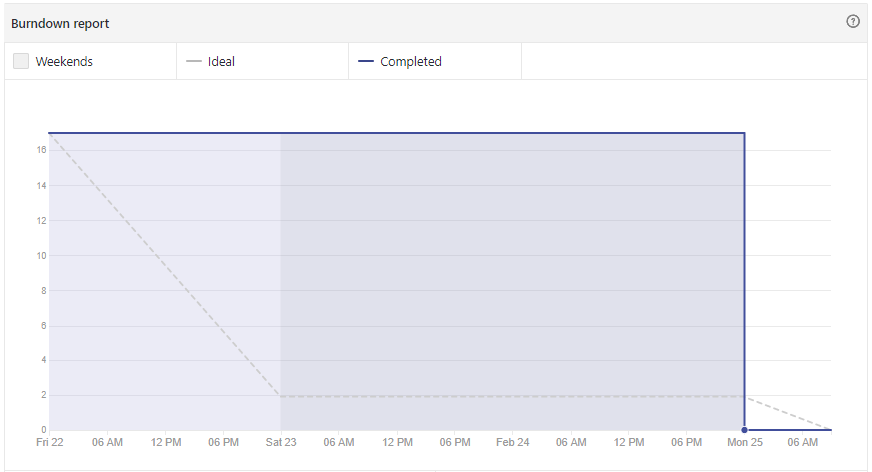
\includegraphics[width=\textwidth]{sprint2}
	\caption{Gráfico del desarrollo del \textit{sprint} 2.}
	\label{fig:sprint2}
\end{figure}

En este \textit{sprint}~\ref{fig:sprint2} se cometió el error contrario al anterior. Éste quizás sea demasiado corto pero aun así se siguió correctamente la planificación inicial.

\subsection{Sprint 3}
Este \textit{sprint} empezó el 25 de Febrero de 2019 y acabó el 7 de Marzo de 2019.

En este \textit{sprint} se quería implementar las funcionalidades de las diferentes pantallas, además de implementar la navegabilidad entre estas.

Las tareas que se realizaron en este \textit{sprint} se resumen en:
\begin{itemize}
	\item Crear las funcionalidades de las distintas pantallas.
	\item Implementar la navegabilidad entre pantallas.
	\item Corrección de \textit{bugs}.
	\item Implementar la generación de comprimidos.
	\item Comentar el código.
\end{itemize}

\begin{figure}
	\centering
	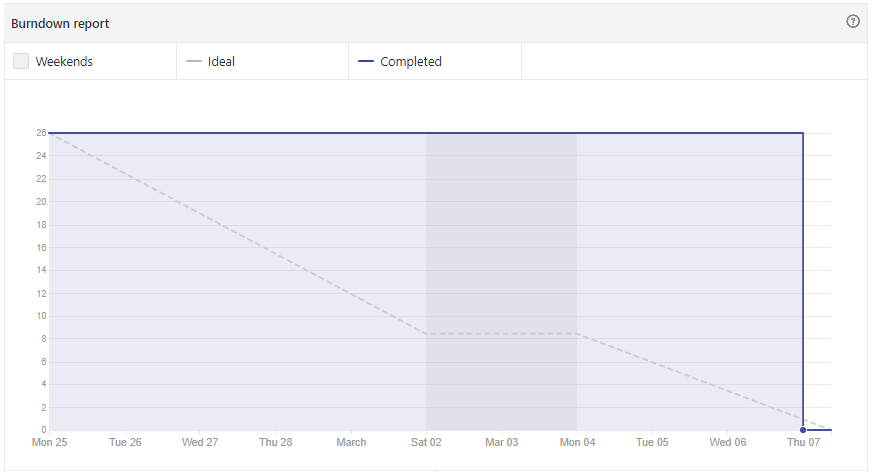
\includegraphics[width=\textwidth]{sprint3}
	\caption{Gráfico del desarrollo del \textit{sprint} 3.}
	\label{fig:sprint3}
\end{figure}

En este \textit{sprint}~\ref{fig:sprint3}, como en el anterior, se consigue correctamente los objetivos en el tiempo que se quería. Esto era esencial, ya que necesitábamos tener la aplicación que nos permitía generar datos lo antes posible para contar con el mayor número de ellos al final del proyecto.

\subsection{Sprint 4}
Este \textit{sprint} comenzó el 7 de Marzo de 2019 y terminó el 18 de Marzo de 2019.

En este \textit{sprint} se quería implementar el método de envío de los comprimidos desde la aplicación según se definiese en la reunión. Además, complementar la aplicación con las emociones y las opciones adicionales que nos tenía que facilitar APACE.

Las tareas que se realizaron en este \textit{sprint} 4 son:
\begin{itemize}
	\item Resumir las opciones adicionales facilitadas por APACE.
	\item Modificación de las pantallas de Estado y de Opciones con los nuevos valores.
	\item Implementación del envío de los comprimidos por correo.
	\item Creación del manual de usuario de la aplicación.
	\item Crear la presentación en \textit{Power Point} para enseñar la aplicación.
	\item Presentación ante familias y cuidadores de la aplicación.
\end{itemize}

\begin{figure}
	\centering
	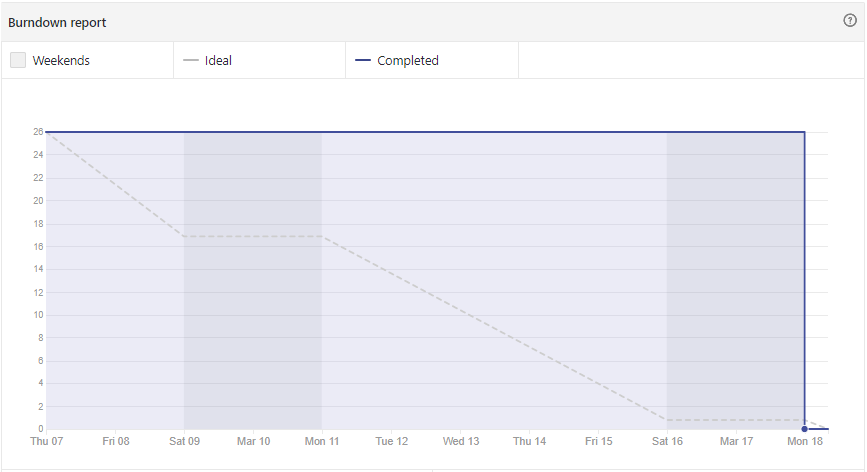
\includegraphics[width=\textwidth]{sprint4}
	\caption{Gráfico del desarrollo del \textit{sprint} 4.}
	\label{fig:sprint4}
\end{figure}

En este \textit{sprint} 4~\ref{fig:sprint4} se han realizado más tareas de las que se pretendía en un principio, ya que no se contaba con tener que hacer la presentación en APACE para mostrar y ayudar a instalar la aplicación.

\subsection{Sprint 5}
Este \textit{sprint} comenzó el 18 de Marzo de 2019 y acabó el 5 de Abril de 2019.

En este \textit{sprint} se pretendía realizar el diseño de la interfaz de la aplicación de interpretación, y generar mis propios datos con la aplicación de generación de datos, ya que como se comentó en la reunión, lo más seguro es que no tuviésemos suficientes datos.

Las tareas del \textit{sprint} 5 se pueden resumir en:
\begin{itemize}
	\item Presentación de la aplicación de generación de datos a las familias que no pudieron estar en la anterior presentación.
	\item Diseño de las posibles interfaces de la aplicación de interpretación.
	\item Diseño de la aplicación.
	\item Elección junto con APACE de la interfaz final.
	\item Generación de mis propios datos.
\end{itemize}

\begin{figure}
	\centering
	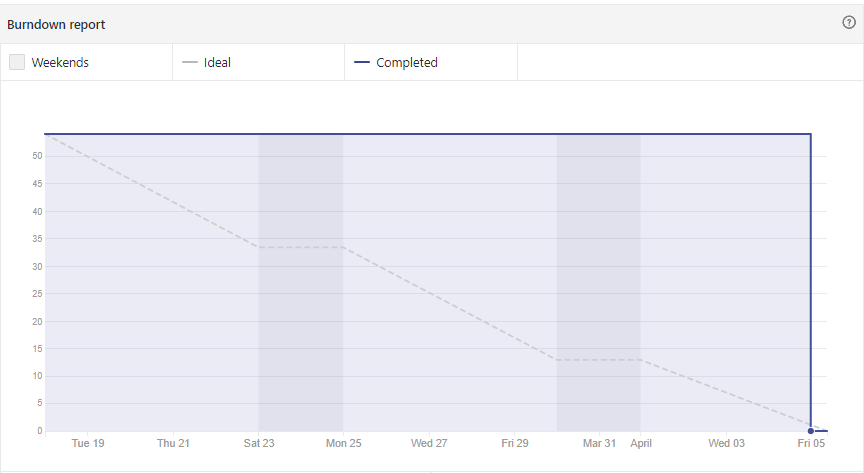
\includegraphics[width=\textwidth]{sprint5}
	\caption{Gráfico del desarrollo del \textit{sprint} 5.}
	\label{fig:sprint5}
\end{figure}

Este \textit{sprint} 5~\ref{fig:sprint5} costó mucho porque la grabación de audios se hizo muy larga, ya que debía de ser precisa. Aun así el \textit{sprint} transcurrió correctamente.

\subsection{Sprint 6}
Este \textit{sprint} comenzó el 5 de Abril de 2019 y terminó el 11 de Abril de 2019.

En este \textit{sprint} se quería, a partir de los diseños hechos en el \textit{sprint} anterior, crear e implementar las funcionalidades de la aplicación de interpretación.

Las tareas que se realizaron en este \textit{sprint} son:
\begin{itemize}
	\item Crear las pantallas y las clases diseñadas.
	\item Implementar las funcionalidades de las clases.
	\item Implementar la navegabilidad entre pantallas.
	\item Modificar las imágenes pasadas por APACE para la accesibilidad.
	\item Implementar el paciente por defecto.
\end{itemize}

\begin{figure}
	\centering
	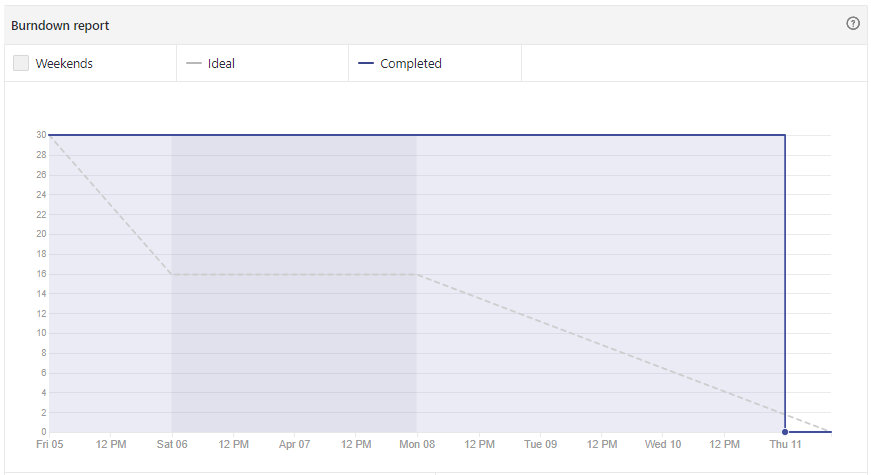
\includegraphics[width=\textwidth]{sprint6}
	\caption{Gráfico del desarrollo del \textit{sprint} 6.}
	\label{fig:sprint6}
\end{figure}

En el \textit{sprint} 6~\ref{fig:sprint6} se ha seguido correctamente la idea inicial de los objetivos marcados para éste.

\subsection{Sprint 7}
Este \textit{sprint} va desde el día 11 de Abril de 2019 hasta el día 28 de Abril de 2019.

En el séptimo \textit{sprint} se quería diseñar e implementar diferentes tipos de test que permitan probar las distintas partes de la aplicación y corregir los \textit{bugs} resultantes.

El resumen de las tareas de este \textit{sprint} es:
\begin{itemize}
	\item Diseño de los test unitarios.
	\item Implementación de los test unitarios.
	\item Diseño de los test de integración.
	\item Implementar los test de integración.
	\item Realizar el \textit{Monkey test}.
	\item Comentar el código de los test.
	\item Corrección de los \textit{bugs} detectados.
\end{itemize}

\begin{figure}
	\centering
	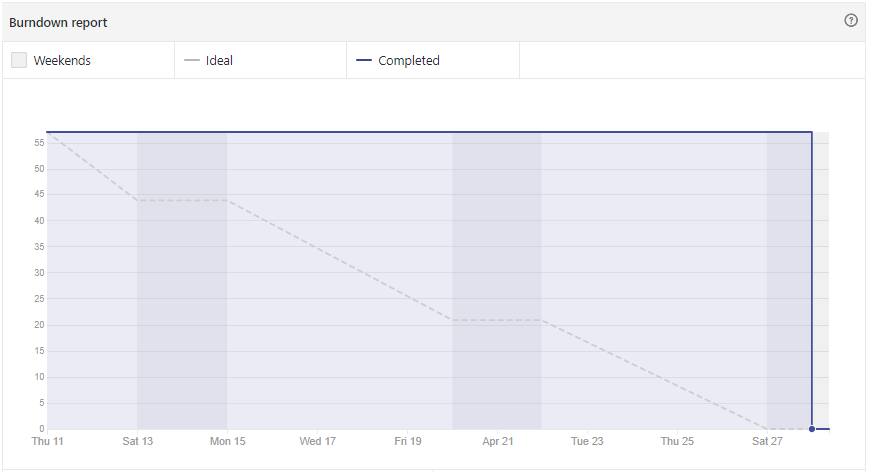
\includegraphics[width=\textwidth]{sprint7}
	\caption{Gráfico del desarrollo del \textit{sprint} 7.}
	\label{fig:sprint7}
\end{figure}

Este ha sido uno de los \textit{sprints} más costosos y a la vez más favorables para el proyecto~\ref{fig:sprint7} ya que, aunque llevó mucho tiempo diseñar e implementar todos los test, dio como resultado encontrar algunos \textit{bugs} que no podría haber detectado de otra manera.

\subsection{Sprint 8}
Este \textit{sprint} se desarrolló desde el 28 de Abril de 2019 hasta el 10 de Mayo de 2019.

En este \textit{sprint} se quería modificar las cosas que nos comentó APACE sobre la interfaz, añadir la pantalla de información, sus test correspondientes y por último comenzar con el diseño del servidor.

Las tareas que finalmente se hicieron fueron:
\begin{itemize}
	\item Cambios en la interfaz pedidos por APACE.
	\item Implementación de la pantalla de información.
	\item Cambios en los diseños, para añadir la nueva información.
	\item Diseño de los test para la pantalla de información.
	\item Implementación de los test de la pantalla de información.
	\item Diseñar el servidor.
	\item Implementar el servidor.
	\item Probar la implementación del servidor.
\end{itemize}

\begin{figure}
	\centering
	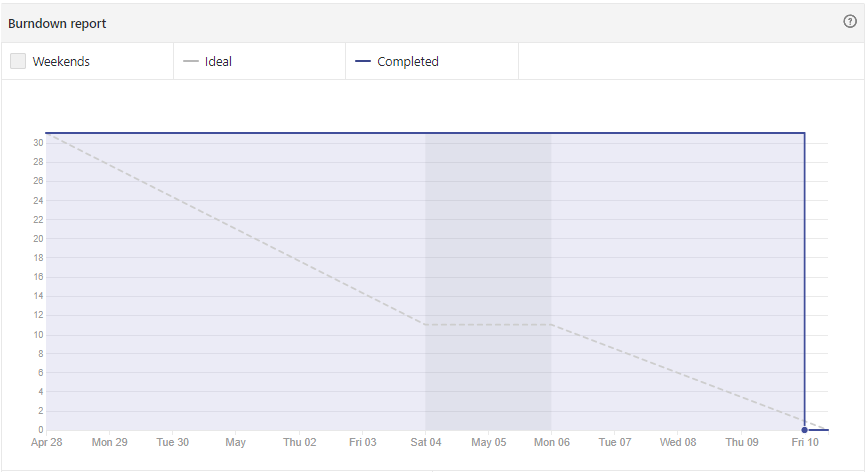
\includegraphics[width=\textwidth]{sprint8}
	\caption{Gráfico del desarrollo del \textit{sprint} 8.}
	\label{fig:sprint8}
\end{figure}

En este \textit{sprint} 8~\ref{fig:sprint8} al final se realizaron todas la tareas que se pretendían y además otras más, sobre todo las tareas de implementación del servidor, que en un principio iba a ser el siguiente \textit{sprint}, pero debido a la necesidad de terminar el servidor lo antes posible se adelantó a éste.

\subsection{Sprint 9}
Este \textit{sprint} comenzó el 10 de Mayo de 2019 y terminó el 17 de Mayo de 2019.

En este \textit{sprint}, que inicialmente se iba a dirigir a desarrollar el servidor \textit{Flask}, se pretendía acabar la implementación de la aplicación desarrollando los métodos \textit{post} al servidor, y crear la presentación y el guión para la presentación del proyecto en conferencia ASPACENet en Madrid.

El conjunto de tareas que se realizaron fueron:
\begin{itemize}
	\item Estudiar como hacer los métodos \textit{post} en \textit{Android}.
	\item Investigar cómo poder conectarse directamente al servidor.
	\item Implementar la conexión entre la aplicación y el servidor.
	\item Comentar el código nuevo.
\end{itemize}

\begin{figure}
	\centering
	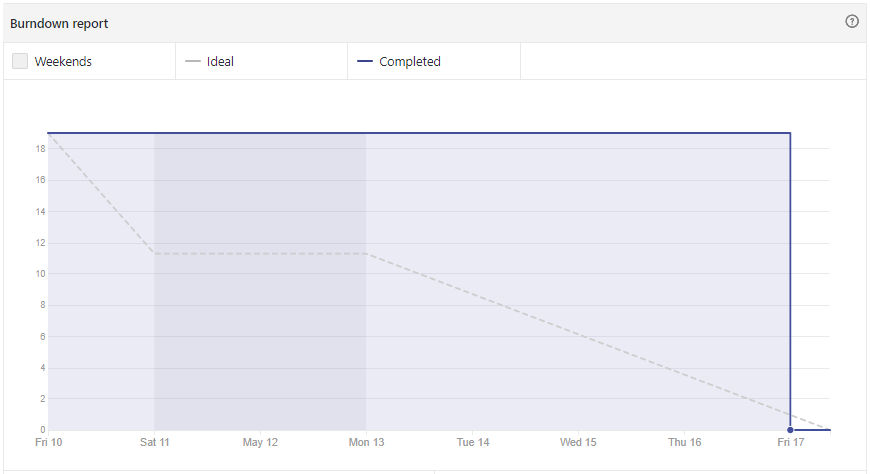
\includegraphics[width=\textwidth]{sprint9}
	\caption{Gráfico del desarrollo del \textit{sprint} 9.}
	\label{fig:sprint9}
\end{figure}

En este \textit{sprint}~\ref{fig:sprint9}, al contrario que en el anterior, no se ha podido realizar todos los objetivos que se tenían, ya que las tareas relacionadas con la creación de la presentación y el guión de Madrid no se han podido hacer.

\subsection{Sprint 10}
 Este \textit{sprint} comenzó el 17 de Mayo de 2019 y terminó el 11 de Junio de 2019.
 
 En este \textit{sprint}, que quería ser el último en el cual hubiese que implementar cosas tanto en las aplicaciones como en el servidor, se quería implementar la descarga del audio en el servidor, cosa que costó mucho. También se quería añadir la parte de clasificación en el servidor con los algoritmos estudiados en los primeros \textit{sprints} y los estudios realizados por el investigador colaborador, Sergio Chico.
 
 La lista resumen de las tareas de este \textit{sprint} es:
 \begin{itemize}
 	\item Desarrollo del paso del audio entre aplicación y servidor con \textit{Base64}.
 	\item Creación dinámica de nombres en el servidor y eliminación al final de los audios.
 	\item Mejorar la visualización del resultado final.
 	\item Elaboración del método que permite devolver un resultado aleatorio.
 	\item Modificación de los test de la aplicación.
 	\item Corrección de \textit{bugs}.
 	\item Creación de la presentación y el guión para Madrid.
 	\item Presentación del proyecto en Madrid.
 	\item Añadir el sistema de predicción en el servidor.
 	\item Crear e implementar el estándar de errores.
 	\item Refactorización de código.
 	\item Grabación del vídeo en APACE.
 	\item Presentación de la aplicación de interpretación a los cuidadores de APACE.
 \end{itemize}

\begin{figure}
	\centering
	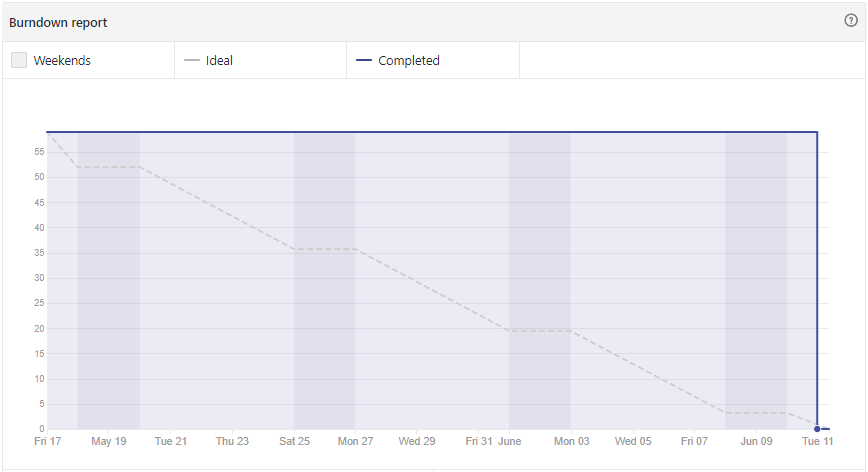
\includegraphics[width=\textwidth]{sprint10}
	\caption{Gráfico del desarrollo del \textit{sprint} 10.}
	\label{fig:sprint10}
\end{figure}

Este \textit{sprint} 10~\ref{fig:sprint10} es sin duda el que más trabajo y problemas ha dado, ya que en él se encuentran varias tareas que han llevado mucho tiempo realizarlas, como por ejemplo la presentación del proyecto en Madrid o el paso del audio al servidor. Aun así, se consiguieron todos los objetivos, sobre todo el de acabar la implementación de las aplicaciones y del servidor.

\subsection{Sprint 11}
Este \textit{sprint} comenzó el 11 de Junio de 2019 y terminó el 18 de Junio de 2019.

En este \textit{sprint} se pretendía presentar el proyecto ante la prensa y empezar la documentación de la memoria.

Las tareas que se realizaron en el \textit{sprint} fueron:
\begin{itemize}
	\item Presentación del proyecto ante la prensa.
	\item Documentación de la memoria.
\end{itemize}

\begin{figure}
	\centering
	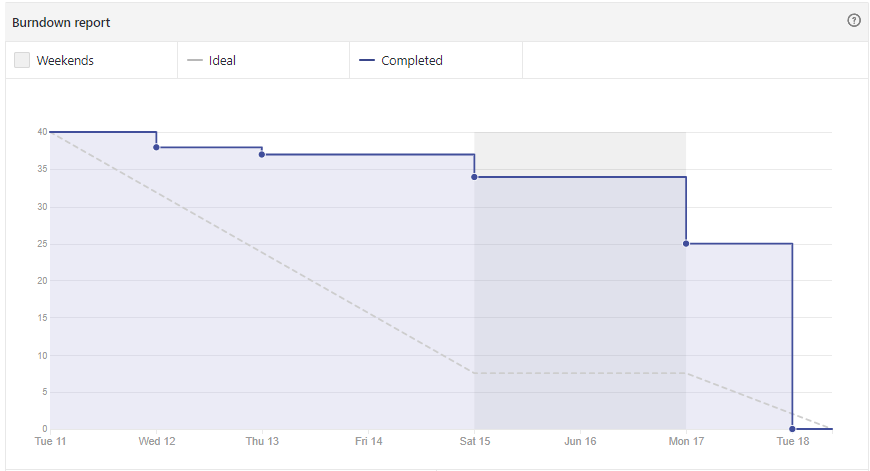
\includegraphics[width=\textwidth]{sprint11}
	\caption{Gráfico del desarrollo del \textit{sprint} 11.}
	\label{fig:sprint11}
\end{figure}

El \textit{sprint} 11~\ref{fig:sprint11} ha sido uno de los más importantes. Se ha cumplido, y con creces, uno de los objetivos que se tenían en el proyecto, este objetivo es la difusión mediática, debido a que gracias a la presentación ante la prensa se obtuvo mucha difusión del proyecto.

\subsection{Sprint 12}
Este \textit{sprint} empezó el 18 de junio de 2019 y acabó el 29 de junio de 29019.

En el \textit{sprint} se pretendía acabar la documentación del proyecto, retocando la memoria y haciendo todos los anexos.

El conjunto de tareas que se realizó en este \textit{sprint} fueron:
\begin{itemize}
	\item Cambios en la memoria solicitados por los tutores.
	\item Elaboración de los anexos.
	\item Grabación de vídeos de la ejecución de las aplicaciones.
	\item Creación de la caratula de los discos.
	\item Generar el \textit{javadoc} de las aplicaciones.
	\item Creación de la portada del repositorio.
\end{itemize}

\begin{figure}
	\centering
	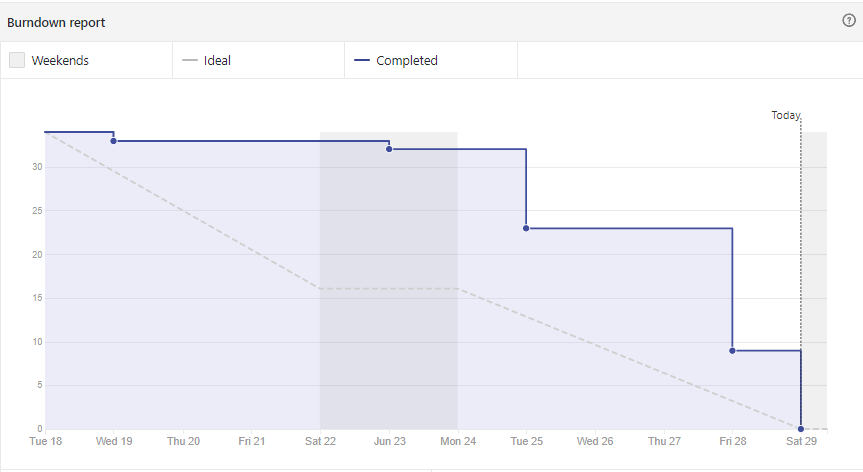
\includegraphics[width=\textwidth]{sprint12}
	\caption{Gráfico del desarrollo del \textit{sprint} 12.}
	\label{fig:sprint12}
\end{figure}

Este \textit{sprint} ha sido el punto y final en la documentación y en la elaboración del proyecto. Aunque el tiempo invertido en tener toda la documentación bien hecha ha sido mucho, como se puede ver en la figura~\ref{fig:sprint12}, el resultado tanto en opinión personal como de mis tutores es más que correcto.

Como se puede observar el proyecto, por mi parte, ha tenido más de 400 horas de trabajo de índole muy distinta. Pero cabe destacar que ese no ha sido el único tiempo invertido en el proyecto, sino que hay que añadir el tiempo de investigación de Sergio Chico y el tiempo invertido en todo el proyecto por mis dos tutores, el doctor César Represa y el doctor José Francisco Díez.
\section{Estudio de viabilidad}
En este apartado se quiere comprobar si la realización del proyecto es posible, teniendo en cuenta los aspectos económicos y legales del mismo.
\subsection{Viabilidad económica}
En este subapartado voy a comentar la viabilidad económica del proyecto, en el cual tenemos que calcular tanto los costes de contratación de las 4 personas del equipo de desarrollo, como los gastos en dispositivos, además de los gastos para las presentaciones del proyecto.

\subsubsection{Coste de personal}
El personal que ha trabajado en este proyecto es muy variado y así hay que tenerlo en cuenta en este apartado. Además, hay que tener en cuenta la duración del proyecto que ha ido desde inicio de Diciembre de 2018 hasta principio de Julio de 2019, un total de 7 meses.

Primero empezaremos con los tutores, donde el coste no lo vamos a calcular por la duración del proyecto sino por los créditos impartidos. En primer lugar tenemos al doctor César Represa Pérez, que es profesor colaborador y por otro lado tenemos al doctor José Francisco Díez Pastor. Al no encontrar datos para los profesores colaboradores se han tomado los valores de ayudante doctor.

El sueldo de un ayudante doctor en la Universidad de Burgos es de 1.842,84\euro al mes~\cite{sueldos}, que daría un total de 22.114,08\euro al año. Teniendo en cuenta que un ayudante doctor tiene que impartir 24 créditos, aunque luego se suele impartir más, el coste por crédito sería de 22.114,08\euro/24 créditos, lo que da un total de 921,42\euro/crédito. Además, sabiendo que el Trabajo Fin de Grado es un total de 1 créditos a repartir entre tutores y tribunal, en este caso vamos a tener en cuenta que el crédito impartido se lo reparten solo los dos tutores, al ser dos tutores serían 0,5 créditos por tutor. Lo que darías un coste total por tutor de 460,71\euro.

Después de calcular el coste de los tutores, paso a calcular el coste de mi compañero investigador y el mio, que van a ser el mismo sueldo por el trabajo de 7 meses. El sueldo mensual neto lo he obtenido del sueldo medio de los empleados en informática~\cite{salario}.

\begin{table}[H]
	\centering
	\begin{tabular}{ll}
		\toprule
		\textbf{Concepto}         & \textbf{Coste}                \\
		\midrule
		Salario mensual neto      & 1.575\euro     \\
		Retención IRPF (15\%)     & 428,76\euro   \\
		Seguridad Social (29,9\%)~\cite{gobees} & 854,67\euro   \\
		Salario mensual bruto     & 2.858,43\euro  \\
		\midrule
		\textbf{Total 7 meses}    & 20.009,01\euro \\		
		\bottomrule
	\end{tabular}
	\caption{Salario trabajador.}
\end{table}

El total de los costes por personal es de:
\begin{table}[H]
	\centering
	\begin{tabular}{ll}
		\toprule
		\textbf{Concepto} & \textbf{Coste} \\ \midrule
		Tutores (x2)      & 921,42\euro   \\
		Trabajadores (x2) & 40.018,02\euro   \\ \midrule
		\textbf{Total}    & 40.939,44\euro   \\ \bottomrule
	\end{tabular}
	\caption{Coste de personal.}
\end{table}

\subsubsection{Coste hardware}
En este apartado voy a calcular el coste de los dispositivos hardware que se han usado a lo largo del desarrollo del proyecto junto con su amortización. Como en la mayoría de los dispositivos hardware, vamos a calcular una armotización de 5 años. En cuanto al coste software no tenemos ningún gasto.

Para el desarrollo he utilizado al menos un dispositivo móvil y dos tablets, y también cuento con la tablet que compraron desde APACE para el proyecto. Además, he usado dos portátiles, pero cuento con el uso de 3 portátiles contando con el ordenador del investigador colaborador.

Las amortizaciones se han calculado por el tiempo usado, es decir, hemos usado todos los dispositivos durante un total de 7 meses.

\begin{table}[H]
	\centering
	\begin{tabular}{lll}
		\toprule
		\textbf{Concepto}        & \textbf{Coste} & \textbf{Amortización} \\ \midrule
		Dispositivo móvil        & 300\euro        & 35\euro                \\
		Dispositivo tablet (x2)  & 700\euro        & 81,67\euro             \\
		Dispositivo tablet APACE & 350\euro        & 40,83\euro             \\
		Ordenadores (x3)         & 2.400\euro       & 280\euro               \\ \midrule
		\textbf{Total}           & 3.750\euro       & 437,5\euro             \\ \bottomrule
	\end{tabular}
	\caption{Coste hardware.}
\end{table}

\subsubsection{Otros gastos}
Como ya he comentado, durante el proyecto hemos tenido otro tipo de gastos para realizar las presentaciones, sobre todo en la presentación de Madrid al cual fuimos 3 personas, estos gastos son:

\begin{table}[H]
	\centering
	\begin{tabular}{ll}
		\toprule
		\textbf{Concepto}       & \textbf{Coste} \\ \midrule
		Desplazamiento a Madrid & 40\euro         \\
		Dietas (x3)             & 36\euro         \\ \midrule
		\textbf{Total}          & 76\euro         \\ \bottomrule
	\end{tabular}
	\caption{Coste del viaje a Madrid.}
\end{table}

\subsubsection{Coste Total}
Una vez hemos desglosado todos los costes del proyecto voy a calcular el coste total de este:

\begin{table}[H]
	\centering
	\begin{tabular}{ll}
		\toprule
		\textbf{Concepto} & \textbf{Coste} \\ \midrule
		Coste de personal & 40.939,44\euro   \\
		Coste hardware    & 3.750\euro       \\
		Otros costes      & 76\euro         \\ \midrule
		\textbf{Total}    & 44.765,44\euro   \\ \bottomrule
	\end{tabular}
	\caption{Coste total.}
\end{table}

Cabe destacar que el proyecto ha sido galardonado con los premios Fundación Vodafone y Becas Prototipo, que han servido para financiar parte de este proyecto. Además, los gastos del viaje a Madrid fueron pagados por APACE. Con todo esto, para que el proyecto sea rentable se necesitaría:

\begin{table}[H]
	\centering
	\begin{tabular}{ll}
		\toprule
		\textbf{Concepto} & \textbf{Coste} \\ \midrule
		Gastos & 44.765,44\euro   \\
		Fundación Vodafone    & -15.000\euro       \\
		Becas Prototipo      & -1.000\euro         \\
		Pagado por APACE      & -76\euro         \\ \midrule
		\textbf{Total}    & 28.689,44\euro   \\ \bottomrule
	\end{tabular}
	\caption{Rentabilidad económica del proyecto.}
\end{table}

\subsection{Viabilidad legal}
En este apartado voy a comentar la viabilidad legal de las licencias de las librerías usadas en el proyecto y la licencia final del proyecto.

Desde el comienzo del proyecto le comunicamos tanto a APACE como a Vodafone que necesitábamos saber la licencia que querían, tanto para que durante el transcurso del desarrollo saber que herramientas podíamos usar, como para obviamente en esta documentación saber que licencia tener. Y aunque se lo preguntásemos en cada una de las reuniones y tras haber enviado varios correos electrónicos a Vodafone, aun no sabemos la licencia que quieren, solo sabemos que quizás sea \textit{open source}. Esto también a afectado al repositorio en \textit{GitHub}, ya que desde un principio lo he tenido que poner en privado, al no saber la licencia del código, pero actualmente lo he modificado a público tras la no respuesta por parte de APACE o Vodafone y por la necesidad de sacar los gráficos del transcurso del desarrollo.

Después de comentar esto, las licencias de las librerías que usamos son:

\begin{table}[H]
	\centering
	\begin{tabular}{ll}
		\toprule
		\textbf{Librería}       & \textbf{Licencia} \\ \hline
		Android Support Library & Apache 2.0        \\
		OpenCSV                 & Apache 2.0        \\
		JavaMail                & GPL v2            \\
		JUnit                   & EPL               \\
		Espresso                & Apache 2.0        \\
		Flask                   & BSD 3 New              \\
		Pandas                  & BSD 3 New            \\
		Numpy                   & BSD 3 New           \\
		Scikit-Learn            & BSD 3 New   \\
		Matplotlib              & PSFL              \\ \bottomrule
	\end{tabular}
	\caption{Licencias de las librerías.}
\end{table}

Además, hemos usado los pictogramas de la pagina de \textit{ARASAAC}~\cite{arasaac}, que tiene un licencia CC BY-NC-SA 3.0 ES. Por lo que las imágenes que he tenido que modificar tienen esta misma licencia.

El uso licencia EPL nos obligaría a descargar las librerías en tiempo de ejecución, ya que no nos permite distribuirlas. Pero, en nuestro caso, la única librería que usa la licencia EPL es \textit{JUnit}, una de las librerías que se usan para probar el código. Como esta no se distribuye junto con el código, no nos obliga a descargarla en tiempo de ejecución.

Tras comprobar las licencias de las librerías que usamos en el proyecto, y ante la negativa de APACE o Vodafone de darnos una respuesta a la pregunta de qué licencia usar, he decidido que la licencia del proyecto sea GPL v3, ya que es la licencia más restrictiva de las herramientas que tengo y me permite en un futuro patentar el software creado.
\apendice{Especificación de Requisitos}

\section{Introducción}
En este anexo se voy a comentar un apartado esencial en el desarrollo de un elemento software, esto es los requisitos funcionales y los casos de uso, ya que representan lo que tiene que ser y/o hacer nuestra aplicación, programa o proyecto en general. Estos conceptos son definidos por el usuario con ayuda de los diseñadores del software, para definir, desde el primer momento, lo que tiene que hacer el software a desarrollar.
\section{Objetivos generales}
Los objetivos generales, expuestos y debatidos en las primeras reuniones con APACE, son los siguientes:
\begin{itemize}
	\item Poder capturar datos con los que poder realizar la investigación.
	\item Interpretar las emociones de los pacientes a partir de grabaciones de audio y unas opciones adicionales.
	\item Interpretar las respuestas de los pacientes a partir de grabaciones de audio.
	\item Toda aplicación desarrollada ha de ser simple y accesible.
\end{itemize}
\section{Catalogo de requisitos}
En esta sección voy a comentar los requisitos funcionales y no funcionales del proyecto.
\subsection{Requisitos funcionales}
\begin{itemize}
	\item \textbf{RF-1 Selección del paciente:} las aplicaciones deben permitir la selección de los pacientes permitidos.
	\begin{itemize}
		\item \textbf{RF-1.1 Visualización de los pacientes:} en las aplicaciones se tiene que poder ver la lista de posible pacientes a seleccionar.
		\item \textbf{RF-1.2 Paciente seleccionado único:} solo se puede seleccionar a un paciente a la vez.
		\item \textbf{RF-1.3 Permanencia del paciente:} en las aplicaciones una vez que se ha seleccionado un paciente este sigue a lo largo de la ejecución, sin variar por ningún tipo de error.
		\item \textbf{RF-1.4 Paciente por defecto:} en la aplicación de interpretación tiene que poder cargarse un paciente por defecto que aparezca seleccionado al abrir la aplicación.
	\end{itemize}
	\item \textbf{RF-2 Selección de emociones/respuestas:} en la aplicación de recogida de datos, el usuario tiene que poder seleccionar las emociones o respuesta relacionado con el sonido que acaba de grabar.
	\begin{itemize}
		\item \textbf{RF-2.1 Selección de emociones o respuesta}: en la aplicación de generación de datos, el usuario solo puede elegir como resultado de la grabación varias emociones o una respuesta, no puede elegir valores de ambos campos.
		\item \textbf{RF-2.2 Selección de sí o no:} en la aplicación de generación de datos, si elegimos como resultado una respuesta esta ha de ser sí o no, pero no se puede seleccionar ambas a la vez.
		\item \textbf{RF-2.3 Selección obligatoria de emociones o respuesta:} en la aplciación de generación de datos, cada grabación tiene que tener asociado al menos una emoción o una respuesta, no se puede enviar una grabación sin resultado.
		\item \textbf{RF-2.4 Carga de datos:} en la aplicación de generación de datos en una misma ejecución sin enviar ni cancelar la ejecución, si hemos seleccionado ya las emociones o la respuesta relacionada, si volvemos a entrar a la pantalla de selección de estas, han de estar cargadas.
	\end{itemize}
	\item \textbf{RF-3 Selección de las opciones adicionales:} el usuario tiene que poder modificar las opciones adicionales del paciente seleccionado.
	\begin{itemize}
		\item \textbf{RF-3.1 Carga de valores:} en la aplicación de generación de datos, el usuario podrá volver a ver las selecciones de las opciones que ha elegido si vuelve a entrar en la pantalla.
		\item \textbf{RF-3.2 Persistencia de las opciones:} en la aplicación de interpretación las opciones de cada cliente se almacenan y se modifican en el servidor, siendo común a todas las ejecuciones.
	\end{itemize}
	\item \textbf{RF-4 Grabación del audio:} el usuario ha de poder grabar los audios.
	\begin{itemize}
		\item \textbf{RF-4.1 Carga del audio grabado:} en la aplicación de generación de datos, un usuario que ya haya grabado una audio lo tendrá cargado en la pantalla de grabación del audio.
		\item \textbf{RF-4.2 Reproducción del audio:} el usuario tiene que poder reproducir el último audio grabado.
		\item \textbf{RF-4.3 Reescritura del audio:} el usuario ha de poder volver a grabar el audio, eliminando el anterior.ç
		\item \textbf{RF-4.4 Reprodución del audio relacionado con el resultado:} el usuario quiere poder escuchar el audio relacionado con el resultado mostrado.
	\end{itemize}
	\item \textbf{RF-5 Subida de los datos:} el usuario quiere poder subir los datos que han generado, para su posterior investigación.
	\item \textbf{RF-6 Interpretación:} el usuario quiere obtener un resultado para el audio que ha grabado.
	\begin{itemize}
		\item \textbf{RF-6.1 Interpretación con paciente entrenado:} el resultado de una interpretación de un cliente, del cual se tiene los modelos de clasificación, ha de ser calculado por estos.
		\item \textbf{RF-6.2 Interpretación con pacientes no entrenados:} el resultado de una interpretación para un cliente sin modelos ha de ser una respuesta aleatoria.
	\end{itemize}
	\item \textbf{RF-7 Ayuda en la ejecución:} el usuario quiere tener información o una ayuda durante la ejecución, para saber que hace cada botón.
	\begin{itemize}
		\item \textbf{RF-7.1 Ayuda con textos en lectura fácil:} cada bóton de la aplicación de interpretación ha de tener un botón de ayuda que abra un diálogo donde se puede leer con texto en lectura fácil lo que hace.
		\item \textbf{RF-7.2 Reproducción de los diálogos:} el usuario quiere que se reproduzcan los textos de los diálogos.
	\end{itemize}
	\item \textbf{RF-8 Información sobre el proyecto:} el usuario quiere ver en la aplicación una pantalla con información sobre el proyecto.
\end{itemize}

\subsection{Requisitos no funcionales}
\begin{itemize}
	\item \textbf{RNF-1 Accesibilidad:} la aplicación de interpretación ha de ser los más accesible posible para que pueda ser usada por el mayor número de personas.
	\item \textbf{RNF-2 Usabilidad:} las aplicaciones han de ser sencillas e intuitivas.
	\item \textbf{RNF-3 Escalabilidad:} el sistema que engloba las aplicaciones y el servidor ha de poder, de forma sencilla, añadir y eliminar pacientes.
	\item \textbf{RNF-4 Disponibilidad:} el servidor ha de ser siempre accesible para poder cargar los pacientes, ver y/o modificar las opciones y para poder interpretar los sonidos.
	\item \textbf{RNF-5 Seguridad:} no ha de poder acceder a los métodos del servidor desde fuera de la aplicación de interpretación de sonidos.
	\item \textbf{RNF-6 Persistencia:} tanto la lista de posibles pacientes, como las opciones de estos y sus modelos de clasificación deben de permanecer accesibles, aunque ocurran problemas de conexión con el servidor.
\end{itemize}

\section{Especificación de requisitos}
Este apartado se va explicar los casos de uso, a partir de diagramas y de tablas.
\subsection{Diagramas de Casos de Uso}
\begin{figure}[H]
	\centering
	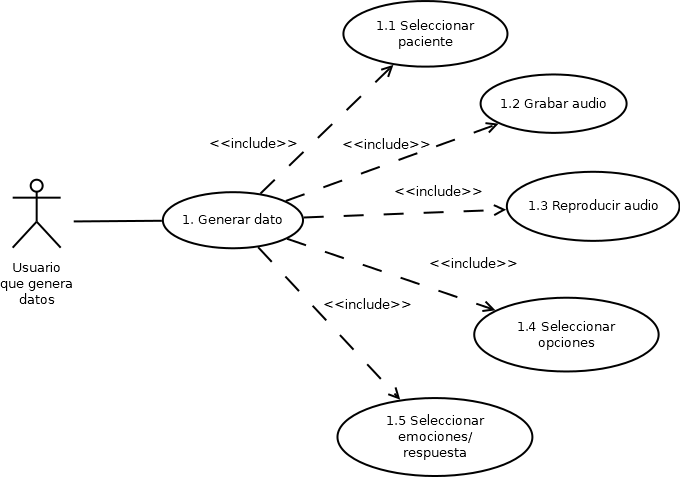
\includegraphics[width=\textwidth]{CU1}
	\caption{Caso de Uso 1.}
	\label{fig:cu1}
\end{figure}

\begin{figure}[H]
	\centering
	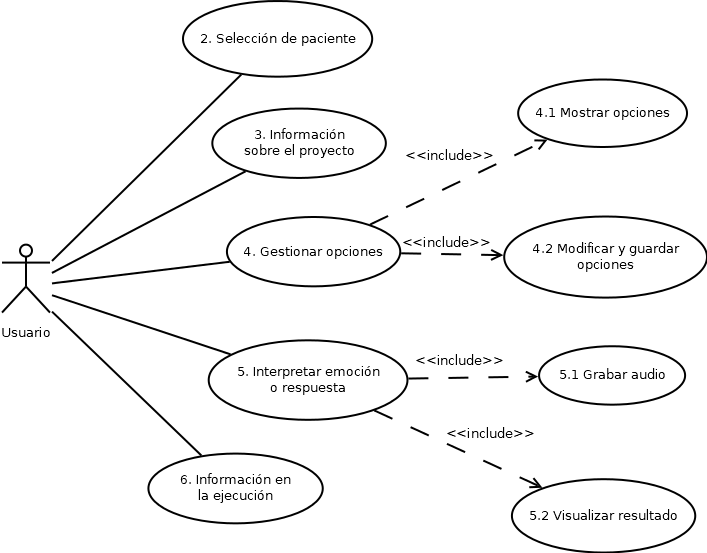
\includegraphics[width=\textwidth]{CU23456}
	\caption{Casos de Uso 2, 3, 4, 5 y 6.}
	\label{fig:cu}
\end{figure}

\subsection{Actores}
Los actores son las personas que interactuan con los elementos desarrollados y son los que definen los casos de uso de un proyecto. En este desarrollo podemos diferenciar los siguiente actores:
\begin{itemize}
	\item \textbf{Usuario que genera datos:} este usuario es el que interacciona con la aplicación para generar datos. Este usuario será los familiares, amigos y cuidadores más cercanos al paciente, que saben interpretar los sonidos que emite.
	\item \textbf{Usuario:} este usuario es el que interacciona con la aplicación de interpretación, y puede ser cualquier tipo de persona que quiera interpretar a una persona con parálisis cerebral gravemente afectada.
\end{itemize}
\subsection{Casos de uso}
\tablaSmallSinColores{Caso de uso 1:	Generar un dato.}{p{3cm} p{.75cm} p{9.5cm}}{tablaCU1}{
	\multicolumn{3}{p{10.25cm}}{\textbf{CU-1: Generar un dato.}} \\
}
{
	\textbf{Descripción}                            & \multicolumn{2}{p{10.25cm}}{El usuario sube un dato generado.} \\\hubu
	\textbf{Requisitos}                         	   & \multicolumn{2}{p{10.25cm}}{RF-5} \\\hubu
	\textbf{Actor}                         	   & \multicolumn{2}{p{10.25cm}}{Usuario que genera un dato.} \\\hubu
	\multirow{3}{3.5cm}{\textbf{Secuencia normal}}  & \textbf{Paso} & \textbf{Acción} \\\cline{2-3}
	& 1    & El usuario accede a la aplicación de generación de datos.\\\cline{2-3}
	& 2	   & El usuario selecciona al paciente. \\\cline{2-3}
	& 3    & El usuario rellena el audio, las opciones y las emociones o respuesta. \\\cline{2-3}
	& 4    & El usuario sube el dato generado. \\\hubu
	\textbf{Postcondiciones}                        & \multicolumn{2}{p{10.25cm}}{El correo con el dato se ha enviado correctamente.} \\\hubu
	\multirow{2}{3.5cm}{\textbf{Excepciones}}       & Paso & Acción \\\cline{2-3}
	& 4    & Si no se tiene conexión a Internet no se envía el dato, pero tampoco se elimina \\\hubu
	\textbf{Frecuencia}                             & Media \\\hubu
	\textbf{Importancia}                            & Crítico \\
}

\tablaSmallSinColores{Caso de uso 1.1:	Seleccionar un paciente.}{p{3cm} p{.75cm} p{9.5cm}}{tablaCU1.1}{
	\multicolumn{3}{p{10.25cm}}{\textbf{CU-1.1: Seleccionar un paciente.}} \\
}
{
	\textbf{Descripción}                            & \multicolumn{2}{p{10.25cm}}{El usuario selecciona y confirma un paciente.} \\\hubu
	\textbf{Precondiciones}                         & \multicolumn{2}{p{10.25cm}}{El usuario se encuentra en el menú principal de la aplicación de recogida de datos} \\\hubu
	\textbf{Requisitos}                         	   & \multicolumn{2}{p{10.25cm}}{RF-1, RF-1.1, RF1.2, RF-1.3.} \\\hubu
	\textbf{Actor}                         	   & \multicolumn{2}{p{10.25cm}}{Usuario que genera un dato.} \\\hubu
	\multirow{3}{3.5cm}{\textbf{Secuencia normal}}  & \textbf{Paso} & \textbf{Acción} \\\cline{2-3}
	& 1    & El usuario accede a la aplicación de generación de datos.\\\cline{2-3}
	& 2	   & El usuario despliega el \textit{spinner} para ver los posibles pacientes. \\\cline{2-3}
	& 3    & El usuario selecciona un paciente de entre los posibles. \\\cline{2-3}
	& 4    & El usuario confirma el paciente pulsando en el botón \textit{SEL.}. \\\hubu
	\textbf{Postcondiciones}                        & \multicolumn{2}{p{10.25cm}}{El usuario ha sido seleccionado y confirmado.} \\\hubu
	\textbf{Frecuencia}                             & Alta \\\hubu
	\textbf{Importancia}                            & Alta \\
}

\tablaSmallSinColores{Caso de uso 1.2:	Grabar audio.}{p{3cm} p{.75cm} p{9.5cm}}{tablaCU1.2}{
	\multicolumn{3}{p{10.25cm}}{\textbf{CU-1.2: Grabar audio.}} \\
}
{
	\textbf{Descripción}                            & \multicolumn{2}{p{10.25cm}}{El usuario graba el sonido emitido por un paciente.} \\\hubu
	\textbf{Precondiciones}                         & \multicolumn{2}{p{10.25cm}}{Hay un paciente seleccionado.} \\\hubu
	\textbf{Requisitos}                         	   & \multicolumn{2}{p{10.25cm}}{RF-4, RF-4.1, RF-4.3} \\\hubu
	\textbf{Actor}                         	   & \multicolumn{2}{p{10.25cm}}{Usuario que genera un dato.} \\\hubu
	\multirow{3}{3.5cm}{\textbf{Secuencia normal}}  & \textbf{Paso} & \textbf{Acción} \\\cline{2-3}
	& 1    & El usuario accede a la aplicación de generación de datos.\\\cline{2-3}
	& 2	   & El usuario selecciona al paciente. \\\cline{2-3}
	& 3    & El usuario pulsa el botón \textit{GRABAR AUDIO}. \\\cline{2-3}
	& 4    & El usuario pulsa el botón \textit{GRABAR} para comenzar a grabar. \\\cline{2-3}
	& 5    & El usuario pulsa el botón \textit{PARAR} para para la grabación.\\\hubu
	\textbf{Postcondiciones}                        & \multicolumn{2}{p{10.25cm}}{El audio está grabado y puede volver a grabarse pulsando el botón "GRABAR".} \\\hubu
	\textbf{Frecuencia}                             & Alta \\\hubu
	\textbf{Importancia}                            & Alta \\
}

\tablaSmallSinColores{Caso de uso 1.3:	Reproducir el audio.}{p{3cm} p{.75cm} p{9.5cm}}{tablaCU1.3}{
	\multicolumn{3}{p{10.25cm}}{\textbf{CU-1.3: Reproducir el audio.}} \\
}
{
	\textbf{Descripción}                            & \multicolumn{2}{p{10.25cm}}{El último audio grabado es reproducido.} \\\hubu
	\textbf{Precondiciones}                         & \multicolumn{2}{p{10.25cm}}{Existe un audio grabado, y el usuario se encuentra en la pantalla de grabación de audio.} \\\hubu
	\textbf{Requisitos}                         	   & \multicolumn{2}{p{10.25cm}}{RF-4.2} \\\hubu
	\textbf{Actor}                         	   & \multicolumn{2}{p{10.25cm}}{Usuario que genera un dato.} \\\hubu
	\multirow{3}{3.5cm}{\textbf{Secuencia normal}}  & \textbf{Paso} & \textbf{Acción} \\\cline{2-3}
	& 1    & El usuario pulsa el botón \textit{REPRODUCIR} y se comienza a reproducir el audio.\\\hubu
	\textbf{Postcondiciones}                        & \multicolumn{2}{p{10.25cm}}{El audio se reproduce, y si se vuelve a pulsar el botón vuelve a comenzar la reproducción.} \\\hubu
	\textbf{Frecuencia}                             & Baja \\\hubu
	\textbf{Importancia}                            & Media \\
}

\tablaSmallSinColores{Caso de uso 1.4:	Seleccionar las opciones adicionales.}{p{3cm} p{.75cm} p{9.5cm}}{tablaCU1.4}{
	\multicolumn{3}{p{10.25cm}}{\textbf{CU-1.4: Seleccionar las opciones adicionales.}} \\
}
{
	\textbf{Descripción}                            & \multicolumn{2}{p{10.25cm}}{El usuario quiere seleccionar las opciones relacionadas con el audio grabado.} \\\hubu
	\textbf{Precondiciones}                         & \multicolumn{2}{p{10.25cm}}{Estamos en la pantalla de selección de opciones y existe un audio grabado.} \\\hubu
	\textbf{Requisitos}                         	   & \multicolumn{2}{p{10.25cm}}{RF-3, RF-3.1} \\\hubu
	\textbf{Actor}                         	   & \multicolumn{2}{p{10.25cm}}{Usuario que genera un dato.} \\\hubu
	\multirow{3}{3.5cm}{\textbf{Secuencia normal}}  & \textbf{Paso} & \textbf{Acción} \\\cline{2-3}
	& 1    & El usuario selecciona las opciones apropiadas en ese momento.\\\hubu
	\textbf{Postcondiciones}                        & \multicolumn{2}{p{10.25cm}}{Las opciones se guardan, y si se vuelve acceder a la pantalla se cargan.} \\\hubu
	\textbf{Frecuencia}                             & Alta \\\hubu
	\textbf{Importancia}                            & Alta \\
}

\tablaSmallSinColores{Caso de uso 1.5:	Seleccionar las emociones o respuestas.}{p{3cm} p{.75cm} p{9.5cm}}{tablaCU1.5}{
	\multicolumn{3}{p{10.25cm}}{\textbf{CU-1: Seleccionar las emociones o respuestas.}} \\
}
{
	\textbf{Descripción}                            & \multicolumn{2}{p{10.25cm}}{El usuario quiere seleccionar las emociones o respuesta relacionadas con el audio.} \\\hubu
	\textbf{Precondiciones}                         & \multicolumn{2}{p{10.25cm}}{Estamos en la pantalla de selección de emociones o respuesta, con un audio grabado y unas opciones seleccionadas.} \\\hubu
	\textbf{Requisitos}                         	   & \multicolumn{2}{p{10.25cm}}{RF-2, RF-2.1, RF-2.2, RF-2.3 y RF-2.4.} \\\hubu
	\textbf{Actor}                         	   & \multicolumn{2}{p{10.25cm}}{Usuario que genera un dato.} \\\hubu
	\multirow{3}{3.5cm}{\textbf{Secuencia normal}}  & \textbf{Paso} & \textbf{Acción} \\\cline{2-3}
	& 1    & El usuario selecciona las emociones o respuesta relacionada.\\\hubu
	\textbf{Postcondiciones}                        & \multicolumn{2}{p{10.25cm}}{Lo seleccionado se guarda, y si se vuelve a entrar en la pantalla se cargarán estos datos.} \\\hubu
	\multirow{2}{3.5cm}{\textbf{Excepciones}}       & Paso & Acción \\\cline{2-3}
	& 1    & Si se selecciona emociones y respuestas no se puede aceptar. \\\cline{2-3} 
	& 1	   & Si se seleccionan las respuestas \textit{sí} y \textit{no}, no se permite aceptar. \\\cline{2-3}
	& 1    & Si no se selecciona nada no deja aceptar y salir de la pantalla.\\\hubu
	\textbf{Frecuencia}                             & Alta \\\hubu
	\textbf{Importancia}                            & Alta \\
}

\tablaSmallSinColores{Caso de uso 2:	Seleccionar paciente.}{p{3cm} p{.75cm} p{9.5cm}}{tablaCU2}{
	\multicolumn{3}{p{10.25cm}}{\textbf{CU-2: Seleccionar paciente.}} \\
}
{
	\textbf{Descripción}                            & \multicolumn{2}{p{10.25cm}}{El usuario selecciona el paciente con el cual quiere trabajar.} \\\hubu
	\textbf{Precondiciones}                         & \multicolumn{2}{p{10.25cm}}{Estar en la aplicación de interpretación, con conexión directa al servidor.} \\\hubu
	\textbf{Requisitos}                         	   & \multicolumn{2}{p{10.25cm}}{RF-1, RF-1.1, RF-1.2, RF-1.3 y RF-1.4} \\\hubu
	\textbf{Actor}                         	   & \multicolumn{2}{p{10.25cm}}{Usuario.} \\\hubu
	\multirow{3}{3.5cm}{\textbf{Secuencia normal}}  & \textbf{Paso} & \textbf{Acción} \\\cline{2-3}
	& 1    & El usuario despliega el \textit{spinner} para ver los posibles pacientes.\\\cline{2-3}
	& 2	   & El usuario selecciona al paciente con el que quiere trabajar.\\\hubu
	\multirow{2}{3.5cm}{\textbf{Excepciones}}       & Paso & Acción \\\cline{2-3}
	& 1	   & Si no se puede conectar con el servidor, saldrá un error 1. \\\hubu
	\textbf{Frecuencia}                             & Alta \\\hubu
	\textbf{Importancia}                            & Alta \\
}

\tablaSmallSinColores{Caso de uso 3:	Obtener información sobre el proyecto.}{p{3cm} p{.75cm} p{9.5cm}}{tablaCU3}{
	\multicolumn{3}{p{10.25cm}}{\textbf{CU-3: Obtener información sobre el proyecto.}} \\
}
{
	\textbf{Descripción}                            & \multicolumn{2}{p{10.25cm}}{El usuario tiene que poder ver información acerca del equipo de desarrollo.} \\\hubu
	\textbf{Precondiciones}                         & \multicolumn{2}{p{10.25cm}}{Estar en la aplicación de interpretación, con conexión directa al servidor.} \\\hubu
	\textbf{Requisitos}                         	   & \multicolumn{2}{p{10.25cm}}{RF-8} \\\hubu
	\textbf{Actor}                         	   & \multicolumn{2}{p{10.25cm}}{Usuario.} \\\hubu
	\multirow{3}{3.5cm}{\textbf{Secuencia normal}}  & \textbf{Paso} & \textbf{Acción} \\\cline{2-3}
	& 1    & El usuario, en el menú principal, pulsa el botón de información al lado del logo de la aplicación.\\\hubu
	\textbf{Postcondiciones}                        & \multicolumn{2}{p{10.25cm}}{El usuario se encuentra en la pantalla de información, puede salir pulsando el botón \textit{Aceptar}.} \\\hubu
	\textbf{Frecuencia}                             & Baja \\\hubu
	\textbf{Importancia}                            & Baja \\
}

\tablaSmallSinColores{Caso de uso 4:	Gestionar las opciones adicionales.}{p{3cm} p{.75cm} p{9.5cm}}{tablaCU4}{
	\multicolumn{3}{p{10.25cm}}{\textbf{CU-4: Gestionar las opciones adicionales.}} \\
}
{
	\textbf{Descripción}                            & \multicolumn{2}{p{10.25cm}}{El usuario quiere gestionar las opciones del paciente seleccionado.} \\\hubu
	\textbf{Precondiciones}                         & \multicolumn{2}{p{10.25cm}}{Estar en la aplicación de interpretación y haber seleccionado al paciente, con conexión directa al servidor.} \\\hubu
	\textbf{Requisitos}                         	   & \multicolumn{2}{p{10.25cm}}{RF-3 y RF-3.2} \\\hubu
	\textbf{Actor}                         	   & \multicolumn{2}{p{10.25cm}}{Usuario.} \\\hubu
	\multirow{3}{3.5cm}{\textbf{Secuencia normal}}  & \textbf{Paso} & \textbf{Acción} \\\cline{2-3}
	& 1    & El usuario, en el menú principal, pulsa el botón de \textit{Registro de Información}.\\\cline{2-3}
	& 2	   & El usuario visualiza las opciones guardadas para el paciente seleccionado. \\\cline{2-3}
	& 3    & El usuario puede modificar y guardar las opciones. \\\hubu
	\multirow{2}{3.5cm}{\textbf{Excepciones}}       & Paso & Acción \\\cline{2-3}
	& 2    &  Si no existe el fichero de opciones en el servidor, este devuelve un error 5.\\\hubu
	\textbf{Frecuencia}                             & Alta \\\hubu
	\textbf{Importancia}                            & Alta \\
}

\tablaSmallSinColores{Caso de uso 4.1:	Mostrar las opciones.}{p{3cm} p{.75cm} p{9.5cm}}{tablaCU4.1}{
	\multicolumn{3}{p{10.25cm}}{\textbf{CU-4.1: Mostrar las opciones.}} \\
}
{
	\textbf{Descripción}                            & \multicolumn{2}{p{10.25cm}}{El usuario al entrar en la pantalla visualizará las opciones guardadas para el paciente seleccionado.} \\\hubu
	\textbf{Precondiciones}                         & \multicolumn{2}{p{10.25cm}}{Estar en la pantalla de opciones.} \\\hubu
	\textbf{Requisitos}                         	   & \multicolumn{2}{p{10.25cm}}{RF-3 y RF-3.2} \\\hubu
	\textbf{Actor}                         	   & \multicolumn{2}{p{10.25cm}}{Usuario.} \\\hubu
	\multirow{3}{3.5cm}{\textbf{Secuencia normal}}  & \textbf{Paso} & \textbf{Acción} \\\cline{2-3}
	& 1    & El usuario visualiza las opciones guardas para el paciente seleccionado.\\\hubu
	\multirow{2}{3.5cm}{\textbf{Excepciones}}       & Paso & Acción \\\cline{2-3}
	& 1    &  Si no existe el fichero de opciones en el servidor, este devuelve un error 5.\\\hubu
	\textbf{Frecuencia}                             & Alta \\\hubu
	\textbf{Importancia}                            & Alta \\
}

\tablaSmallSinColores{Caso de uso 4.2:	Modificar y guardar las opciones.}{p{3cm} p{.75cm} p{9.5cm}}{tablaCU4.2}{
	\multicolumn{3}{p{10.25cm}}{\textbf{CU-4.2: Modificar y guardar las opciones.}} \\
}
{
	\textbf{Descripción}                            & \multicolumn{2}{p{10.25cm}}{El usuario modifica, y guarda o cancela los cambios.} \\\hubu
	\textbf{Precondiciones}                         & \multicolumn{2}{p{10.25cm}}{Estar en la pantalla de opciones.} \\\hubu
	\textbf{Requisitos}                         	   & \multicolumn{2}{p{10.25cm}}{RF-5} \\\hubu
	\textbf{Actor}                         	   & \multicolumn{2}{p{10.25cm}}{Usuario.} \\\hubu
	\multirow{3}{3.5cm}{\textbf{Secuencia normal}}  & \textbf{Paso} & \textbf{Acción} \\\cline{2-3}
	& 1    & El usuario visualiza las opciones para el paciente seleccionado.\\\cline{2-3}
	& 2	   & El usuario modifica alguna de las opciones, habilitando así el botón \textit{Guardar}. \\\cline{2-3}
	& 3    & El usuario guarda o cancela los cambios. \\\hubu
	\textbf{Postcondiciones}                        & \multicolumn{2}{p{10.25cm}}{Si el usuario ha decidido guardar, los cambios se realizan en el servidor.} \\\hubu
	\multirow{2}{3.5cm}{\textbf{Excepciones}}       & Paso & Acción \\\cline{2-3}
	& 1    &  Si no existe el fichero de opciones en el servidor, este devuelve un error 5.\\\cline{2-3}
	& 3    & Si no hay conexión con el servidor, se muestra un error 1. \\\hubu
	\textbf{Frecuencia}                             & Media \\\hubu
	\textbf{Importancia}                            & Alta \\
}

\tablaSmallSinColores{Caso de uso 5:	Interpretar emoción o respuesta.}{p{3cm} p{.75cm} p{9.5cm}}{tablaCU5}{
	\multicolumn{3}{p{10.25cm}}{\textbf{CU-5: Interpretar emoción o respuesta.}} \\
}
{
	\textbf{Descripción}                            & \multicolumn{2}{p{10.25cm}}{El usuario quiere interpretar las emociones y las respuestas de los pacientes.} \\\hubu
	\textbf{Precondiciones}                         & \multicolumn{2}{p{10.25cm}}{Estar en la aplicación de interpretación con un paciente seleccionado, y con conexión directa al servidor.} \\\hubu
	\textbf{Requisitos}                         	   & \multicolumn{2}{p{10.25cm}}{RF-6, RF-6.1 y RF-6.2.} \\\hubu
	\textbf{Actor}                         	   & \multicolumn{2}{p{10.25cm}}{Usuario.} \\\hubu
	\multirow{3}{3.5cm}{\textbf{Secuencia normal}}  & \textbf{Paso} & \textbf{Acción} \\\cline{2-3}
	& 1    & El usuario, en el menú principal, pulsa el botón \textit{Qué quiero decir}.\\\cline{2-3}
	& 2	   & El usuario selecciona el tipo de interpretación que quiere hacer. \\\cline{2-3}
	& 3    & El usuario graba el audio que quiere interpretar. \\\cline{2-3}
	& 4    & El usuario visualiza y escucha el resultado. \\\hubu
	\multirow{2}{3.5cm}{\textbf{Excepciones}}       & Paso & Acción \\\cline{2-3}
	& 1    & Si no se puede conectar con el servidor, saldrá un error 1. \\\cline{2-3}
	& 4	   & Si no se puede conectar con el servidor, saldrá un error 1.\\\cline{2-3}
	& 4    & Si no existe un modelo válido para el paciente error 8. \\\hubu
	\textbf{Frecuencia}                             & Alta \\\hubu
	\textbf{Importancia}                            & Crítica \\
}

\tablaSmallSinColores{Caso de uso 5.1:	Grabar audio.}{p{3cm} p{.75cm} p{9.5cm}}{tablaCU5.1}{
	\multicolumn{3}{p{10.25cm}}{\textbf{CU-5.1: Grabar audio.}} \\
}
{
	\textbf{Descripción}                            & \multicolumn{2}{p{10.25cm}}{El usuario tiene que poder grabar el audio que quiere interpretar.} \\\hubu
	\textbf{Precondiciones}                         & \multicolumn{2}{p{10.25cm}}{Haber seleccionado un paciente, y estar en la pantalla de selección de interpretación con conexión directa al servidor.} \\\hubu
	\textbf{Requisitos}                         	   & \multicolumn{2}{p{10.25cm}}{RF-5} \\\hubu
	\textbf{Actor}                         	   & \multicolumn{2}{p{10.25cm}}{Usuario.} \\\hubu
	\multirow{3}{3.5cm}{\textbf{Secuencia normal}}  & \textbf{Paso} & \textbf{Acción} \\\cline{2-3}
	& 1    & El usuario selecciona el tipo de interpretación.\\\cline{2-3}
	& 2	   & El usuario graba el audio que quiere interpretar.\\\hubu
	\textbf{Postcondiciones}                        & \multicolumn{2}{p{10.25cm}}{El audio que ha grabado se puede reproducir, pulsando el botón \textit{Escuchar}, o se puede volver a grabar pulsando \textit{Grabar}.} \\\hubu
	\textbf{Frecuencia}                             & Alta \\\hubu
	\textbf{Importancia}                            & Crítica \\
}

\tablaSmallSinColores{Caso de uso 5.2:	Visualizar y escuchar el resultado.}{p{3cm} p{.75cm} p{9.5cm}}{tablaCU5.2}{
	\multicolumn{3}{p{10.25cm}}{\textbf{CU-5.2: Visualizar y escuchar el resultado.}} \\
}
{
	\textbf{Descripción}                            & \multicolumn{2}{p{10.25cm}}{El usuario quiere visualizar el resultado y poder volver a escuchar el audio relacionado con este resultado.} \\\hubu
	\textbf{Precondiciones}                         & \multicolumn{2}{p{10.25cm}}{Estar en la pantalla de grabación del audio, con un audio ya grabado y con conexión directa al servidor.} \\\hubu
	\textbf{Requisitos}                         	   & \multicolumn{2}{p{10.25cm}}{RF-6, RF-6.1, RF-6.2 y RF-4.4.} \\\hubu
	\textbf{Actor}                         	   & \multicolumn{2}{p{10.25cm}}{Usuario.} \\\hubu
	\multirow{3}{3.5cm}{\textbf{Secuencia normal}}  & \textbf{Paso} & \textbf{Acción} \\\cline{2-3}
	& 1    & El usuario pulsa el botón \textit{Entender} para ver el resultado.\\\cline{2-3}
	& 2	   & El usuario visualiza y escucha el resultado. \\\cline{2-3}
	& 3    & El usuario puede volver a escuchar el audio relacionado con ese resultado pulsando el botón \textit{Escuchar}. \\\hubu
	\textbf{Postcondiciones}                        & \multicolumn{2}{p{10.25cm}}{El correo con el dato se ha enviado correctamente.} \\\hubu
	\multirow{2}{3.5cm}{\textbf{Excepciones}}       & Paso & Acción \\\cline{2-3}
	& 2    & Si no se tiene conexión con el servidor, error 1. \\\cline{2-3}
	& 2    & Si no existe el modelo entrenado o está dentro del grupo de resultado aleatorios, error 8. \\\hubu
	\textbf{Frecuencia}                             & Alta \\\hubu
	\textbf{Importancia}                            & Crítica \\
}

\tablaSmallSinColores{Caso de uso 6:	Información en la ejecución.}{p{3cm} p{.75cm} p{9.5cm}}{tablaCU6}{
	\multicolumn{3}{p{10.25cm}}{\textbf{CU-6: Información en la ejecución.}} \\
}
{
	\textbf{Descripción}                            & \multicolumn{2}{p{10.25cm}}{El usuario quiere tener información sobre las acciones que hacen los botones de la aplicación.} \\\hubu
	\textbf{Precondiciones}                         & \multicolumn{2}{p{10.25cm}}{-} \\\hubu
	\textbf{Requisitos}                         	   & \multicolumn{2}{p{10.25cm}}{RF-5} \\\hubu
	\textbf{Actor}                         	   & \multicolumn{2}{p{10.25cm}}{Usuario.} \\\hubu
	\multirow{3}{3.5cm}{\textbf{Secuencia normal}}  & \textbf{Paso} & \textbf{Acción} \\\cline{2-3}
	& 1    & Si el usuario pulsa algún botón de información se abrirá un diálogo explicativo en lectura fácil, además se reproducirá por audio. \\\hubu
	\textbf{Frecuencia}                             & Baja \\\hubu
	\textbf{Importancia}                            & Baja \\
}
\apendice{Especificación de diseño}

\section{Introducción}

\section{Diseño de datos}

\section{Diseño procedimental}

\section{Diseño arquitectónico}



\apendice{Documentación técnica de programación}

\section{Introducción}

\section{Estructura de directorios}

\section{Manual del programador}

\section{Compilación, instalación y ejecución del proyecto}

\section{Pruebas del sistema}

\apendice{Documentación de usuario}

\section{Introducción}
En este apartado se comenta una parte esencial dentro de la documentación de un proyecto, los manuales de usuario. Estos son documentos donde los desarrolladores tienen que poner toda la información necesaria para instalar y ejecutar los programas y/o aplicaciones que han desarrollado. Estos documentos tienen que tener también los requisitos que se necesitan para poder instalar y ejecutar los programas, e incluso pueden incluir comentarios que nos dicen que hacer en caso de error de la aplicación.

Este apartado ha sido dividido por los distintos manuales de las distintas aplicaciones que he hecho, de cada una se comentarán los requisitos de los usuarios, la instalación y como se ejecuta. Estas aplicaciones de las que vamos a hablar son:
\begin{itemize}
	\item \textbf{Aplicación de grabación prototipo:} aplicación que un principio iba a ser la aplicación con la cual generar datos. Nos permite grabar audios con el nombre que elijamos.
	\item \textbf{Aplicación para la recogida de datos:} aplicación final para la recogida que nos permite grabar un audio y seleccionar tanto las opciones adicionales como las emociones o respuesta relacionada.
	\item \textbf{Aplicación para la interpretación:} aplicación final AVC que nos permite modificar las opciones adicionales de los pacientes comunes a todos los dispositivos y nos permite interpretar una emoción o una respuesta.
\end{itemize}
\section{Aplicación de grabación prototipo}
\subsection{Uso}
Este es un prototipo de la aplicación final, en este prototipo se permite grabar y dar nombre a audios y reproducirlos.

Estos audios se almacenan en un carpeta llamada Apace localizada en la raíz.

\subsection{Requisitos}
El requisito principal es contar con un dispositivo \textit{smartphone Android} actualizado, con versión \textit{Android} 6.0 o superior.

\subsubsection{Instalación}
Para poder instalar la aplicación el único requisito que se necesita es conexión a Internet para poder descargarse la aplicación.

\subsubsection{Ejecución}
Para la ejecución del prototipo solo se requiere que la aplicación esté instalada y que se acepten los permisos de grabación de audio y de escritura que se preguntan al principio de la ejecución.

\subsection{Instalación}
La instalación del prototipo es sencilla, solo hay que descargar el archivo \textit{apk} desde donde se haya sido suministrado (correo, \textit{WhatsApp}, \textit{GitHub}) y realizar los ajustes necesarios para poder descargarla al ser una aplicación ajena a \textit{Play Store}.

Estos ajustes adicionales consisten simplemente aceptar que se descargue esta aplicación exterior a \textit{Play Store}.

Una vez descargada el \textit{apk} de la aplicación aparecerá en su menú de aplicaciones instaladas con el nombre de Apace, como se puede ver en la figura~\ref{fig:logopro}.

\begin{figure}[H]
	\centering
	
\includegraphics[scale=0.6]{logopro}
	\caption{Logotipo y nombre de la aplicación una vez instalada.}
	\label{fig:logopro}
\end{figure}

\subsection{Ejecución}
Para la ejecución solo tenemos que pulsar el logotipo anteriormente mostrado. En la primera ejecución que hagamos del prototipo nos saldrá el siguiente diálogo, para pedirnos permisos para poder usar tanto el sistema de grabación de audio, como para poder almacenar archivos. Debemos dar permisos a ambos pulsando en la opción \textit{Permitir}. Es muy importante aceptar estos permisos ya que sino la aplicación se cerrará en la primera vez que queramos grabar un audio. En cualquier caso si por algún error se ha denegado los permisos y la aplicación se ha cerrado se puede volver a abrir y nos volverá a pedir aceptar los permisos. La petición de estos permisos se pueden ver en las figuras~\ref{fig:properr1} y ~\ref{fig:proper2}.

\begin{figure}[H]
	\centering
	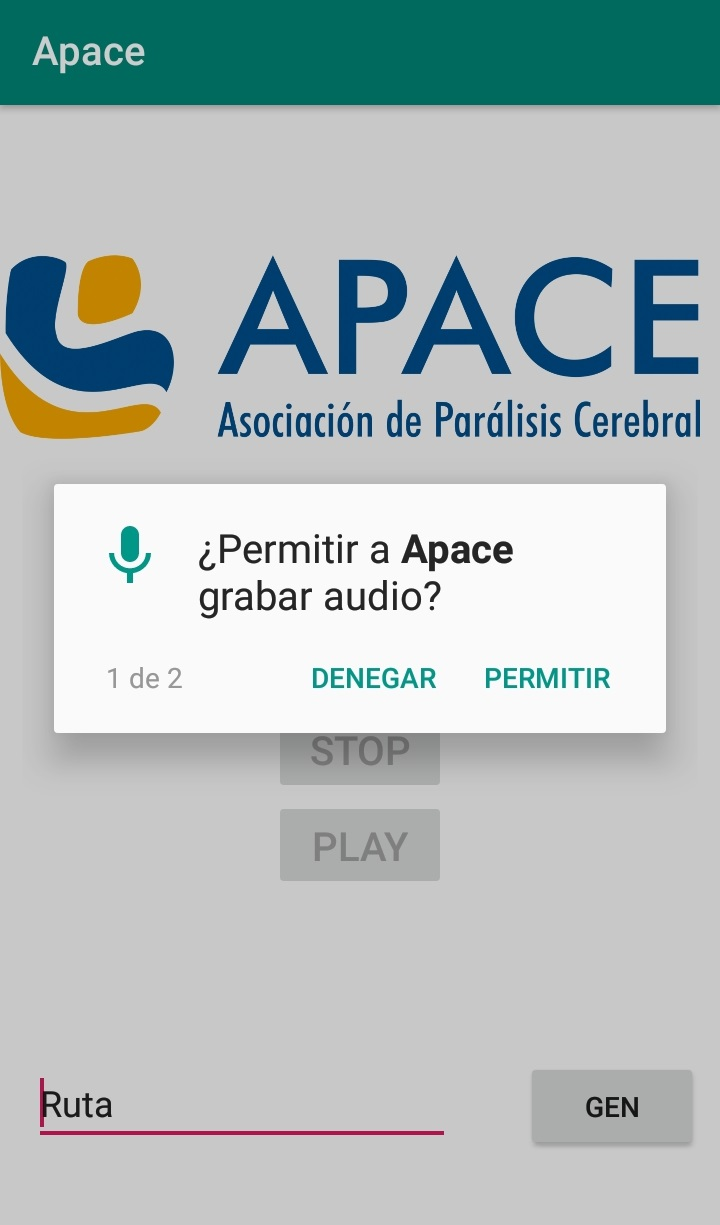
\includegraphics[scale=0.3]{proper1}
	\caption{Petición de permisos para la grabación de audio.}
	\label{fig:properr1}
\end{figure}

\begin{figure}[H]
	\centering
	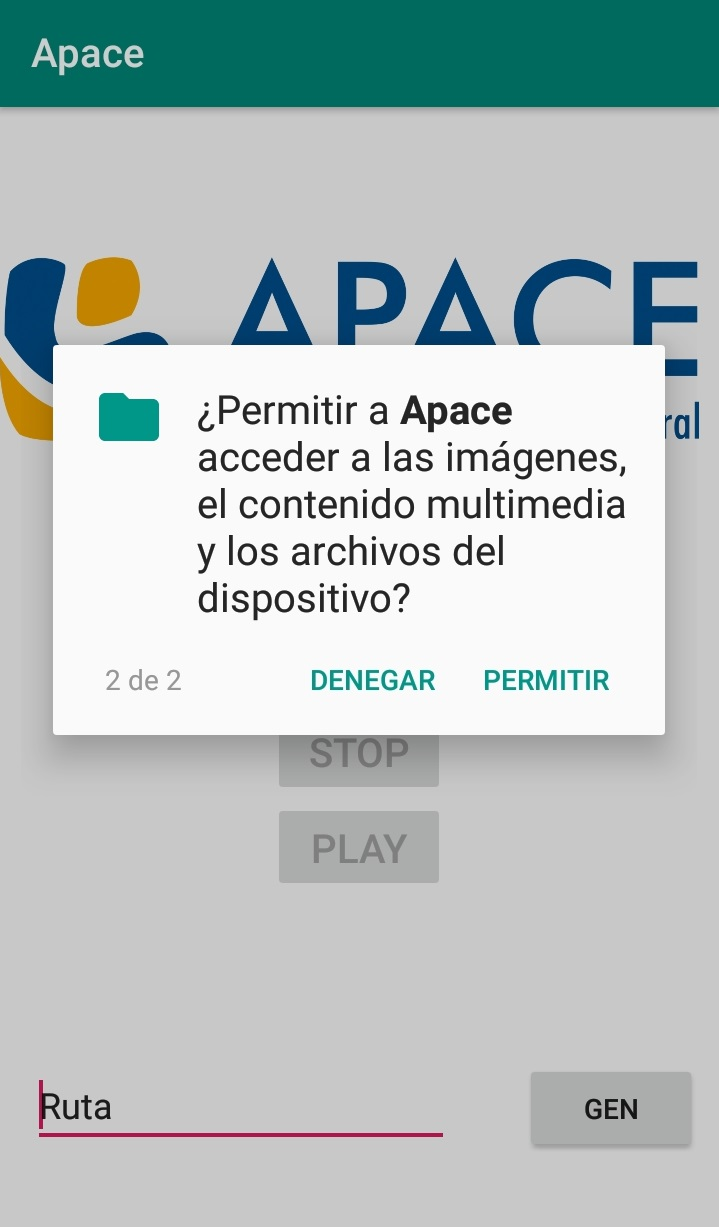
\includegraphics[scale=0.3]{proper2}
	\caption{Petición de permisos para el acceso al almacenamiento multimedia.}
	\label{fig:proper2}
\end{figure}

Después de aceptar los permisos tendremos acceso al menú principal de la aplicación, como se ve en la figura~\ref{fig:promp}, en el se pueden ver 3 botones (\textit{RECORD}, \textit{STOP} y \textit{PLAY}) y una caja de texto con un botón \textit{GEN}.

\begin{figure}[H]
	\centering
	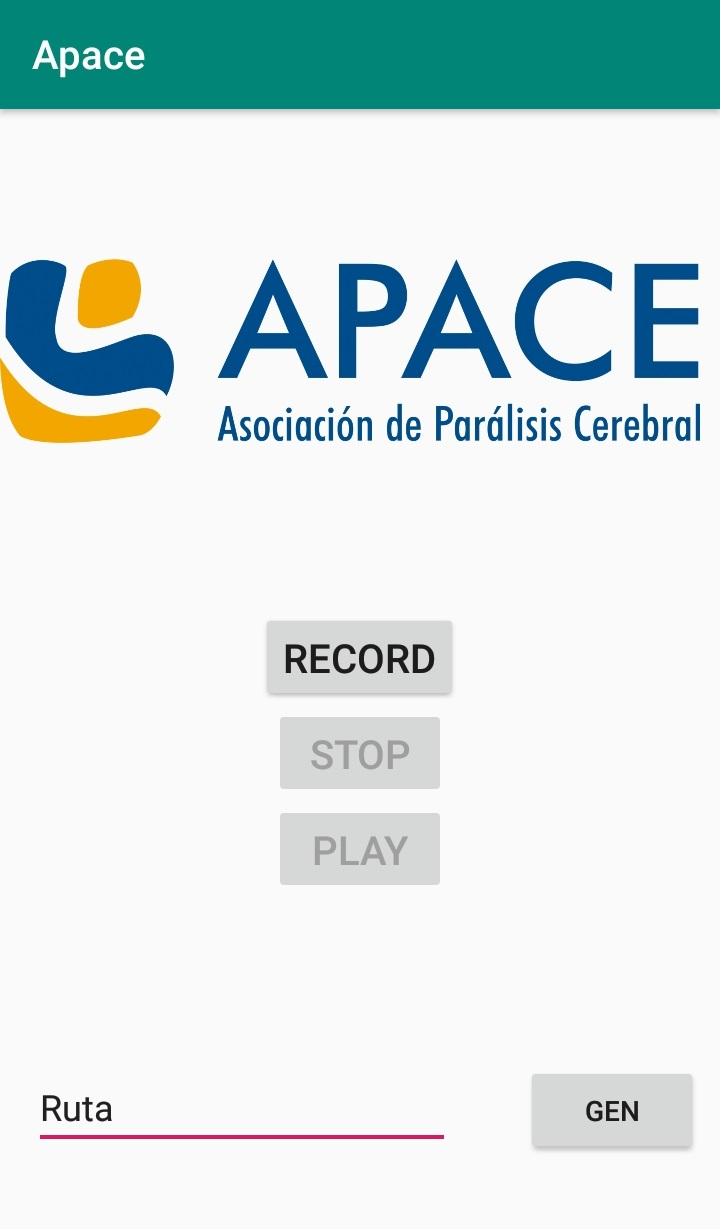
\includegraphics[scale=0.3]{promp}
	\caption{Menú principal de la aplicación prototipo.}
	\label{fig:promp}
\end{figure}

Los tres primeros botones sirven para manejar la grabación de los audios, al principio solo tendremos habilitado el botón \textit{RECORD} que nos permite comenzar a grabar el audio siempre que la caja de texto no esté vacía o que en ella haya un nombre que ya existe (es decir, que ya exista un audio con ese nombre).

Una vez pulsemos el botón \textit{RECORD} este quedará deshabilitado y se habilitará el botón \textit{STOP} que nos permite parar y guardar la grabación.

Cuando hayamos finalizado la grabación se nos habilitarán los botones de \textit{RECORD} para poder volver a grabar y de \textit{PLAY} que nos permite reproducir el audio con el nombre que esté en la caja de texto de la ruta (nombre del archivo).

Por último tenemos la caja de texto con la ruta donde podremos elegir el nombre que le queremos dar al archivo o podemos generarlo automáticamente con el botón \textit{GEN} que generará un nombre con la hora y fecha de la grabación.
\section{Aplicación para la recogida de datos}
\subsection{Uso}
Esta aplicación sirve para recolectar datos necesarios para realizar la investigación y la creación de la aplicación final de predicción de emociones y respuestas. Esta aplicación nos permite grabar a los pacientes y tras rellenar dos formularios, genera un archivo comprimido con la grabación de audio y las respuestas de los formularios, y lo envía para que se pueda realizar la investigación.
\subsection{Requisitos}
El requisito principal es contar con un dispositivo \textit{smartphone Android} actualizado, con versión \textit{Android} 6.0 o superior, y conexión a Internet ya sea vía \textit{Wi-Fi} o datos móviles.

\subsubsection{Instalación}
Para poder instalar la aplicación el único requisito que se necesita es conexión a Internet para poder descargarse la aplicación.
\subsubsection{Ejecución}
Para la ejecución del prototipo se requiere que la aplicación esté instalada, que se acepten los permisos de grabación de audio y de escritura que se preguntan al principio de la ejecución y conexión a Internet para poder subir los archivos grabados.

\subsection{Instalación}
La instalación del prototipo es sencilla, solo hay que descargar el archivo \textit{apk} desde donde se haya sido suministrado (correo, \textit{WhatsApp}, \textit{GitHub}) y realizar los ajustes necesarios para poder descargarla al ser una aplicación ajena a \textit{Play Store}.

Estos ajustes adicionales consisten simplemente aceptar que se descargue esta aplicación exterior a \textit{Play Store}.

Una vez descargada la \textit{apk} la aplicación aparecerá en su menú de aplicaciones instaladas con el nombre de AplicaciónGSAudios, como se puede ver en la figura~\ref{fig:logogd}.

\begin{figure}[H]
	\centering
	
\includegraphics[scale=0.6]{logogd}
	\caption{Logotipo y nombre de la aplicación de generación de datos.}
	\label{fig:logogd}
\end{figure}

\subsection{Ejecución}
Para la ejecución solo tenemos que seleccionar el logotipo anteriormente mostrado. En la primera ejecución que hagamos del prototipo nos saldrá el siguiente diálogo para pedirnos permisos para poder usar tanto el sistema de grabación de audio como para poder almacenar archivos, debemos dar permisos a ambos pulsando en la opción \textit{Permitir}, es muy importante aceptar estos permisos ya que sino la aplicación se cerrará en la primera vez que queramos grabar un audio. En cualquier caso, si por algún error se ha denegado los permisos y la aplicación se ha cerrado se puede volver a abrir y nos volverá a pedir aceptar los permisos. La petición de estos permisos se puede ver en las figuras~\ref{fig:gdper1} y ~\ref{fig:gdper2}.

\begin{figure}[H]
	\centering
	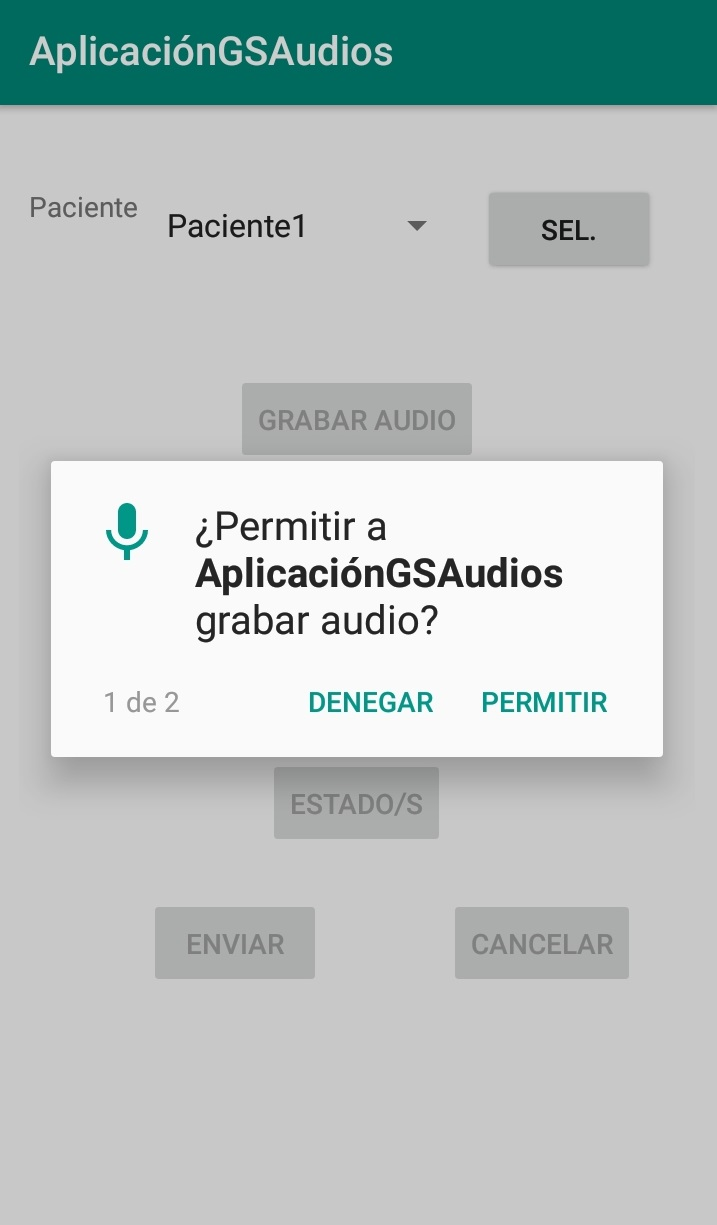
\includegraphics[scale=0.3]{gdper1}
	\caption{Petición de permisos para la grabación de audio en la aplicación de recogida de datos.}
	\label{fig:gdper1}
\end{figure}

\begin{figure}[H]
	\centering
	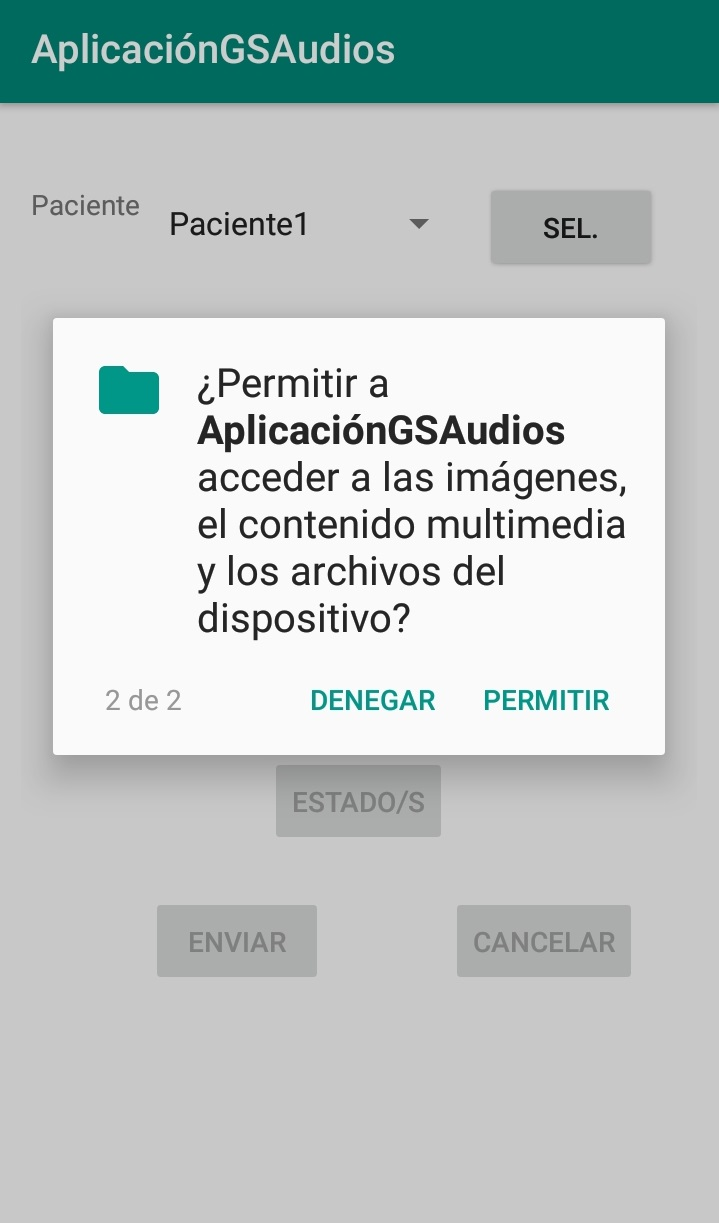
\includegraphics[scale=0.3]{gdper2}
	\caption{Petición de permisos para el acceso al almacenamiento multimedia en la aplicación de recogida de datos.}
	\label{fig:gdper2}
\end{figure}

Después de aceptar los permisos tendremos acceso al menú principal de la aplicación, como se puede ver en la figura~\ref{fig:mpgd}, en la parte superior de este, se puede ver la selección del paciente sobre el cual vamos a realizar la grabación.

\begin{figure}[H]
	\centering
	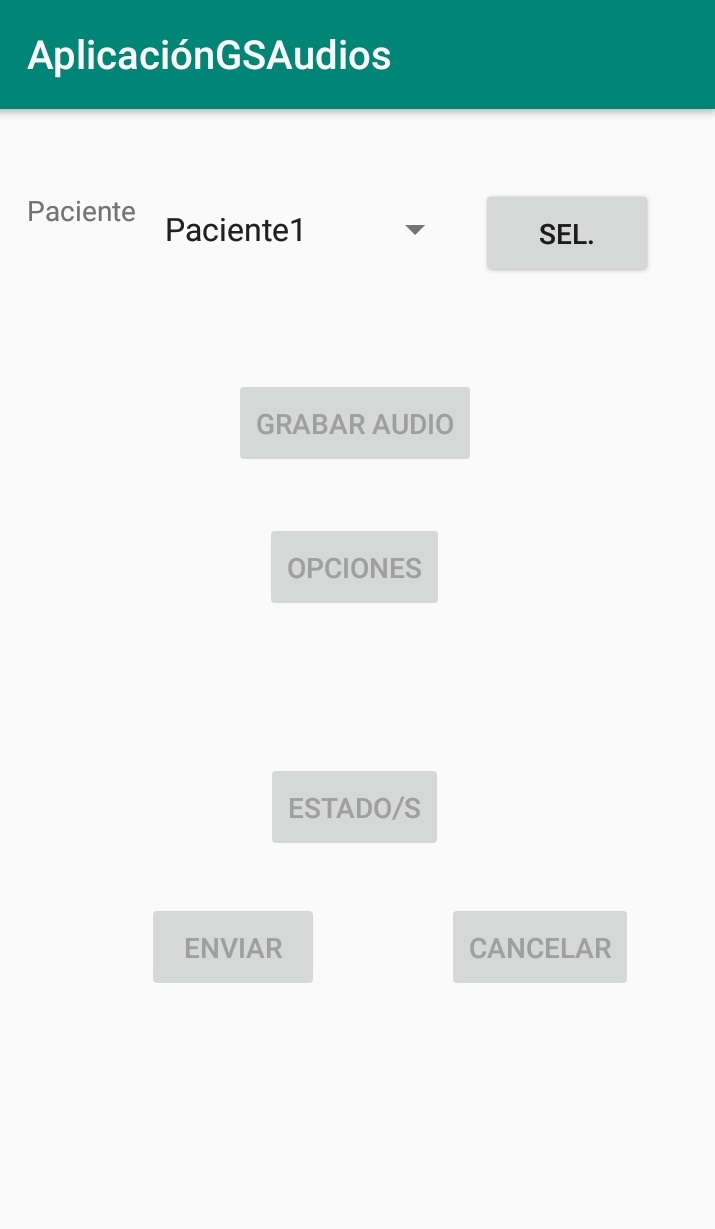
\includegraphics[scale=0.3]{mpgd}
	\caption{Menú principal de la aplicación para la recogida de datos.}
	\label{fig:mpgd}
\end{figure}

Tras haber seleccionado al paciente sobre el cual se va a recoger los datos debemos confirmar la selección del paciente pulsando el botón \textit{Sel.} (Seleccionar). Tras pulsar el botón \textit{Sel.} se nos habilitará el botón \textit{Grabar Audio}, en todo momento desde la pantalla del menú principal podremos cancelar la grabación y la selección del paciente pulsando el botón \textit{Cancelar}, como se puede ver en la figura~\ref{fig:mp2gd}.

\begin{figure}[H]
	\centering
	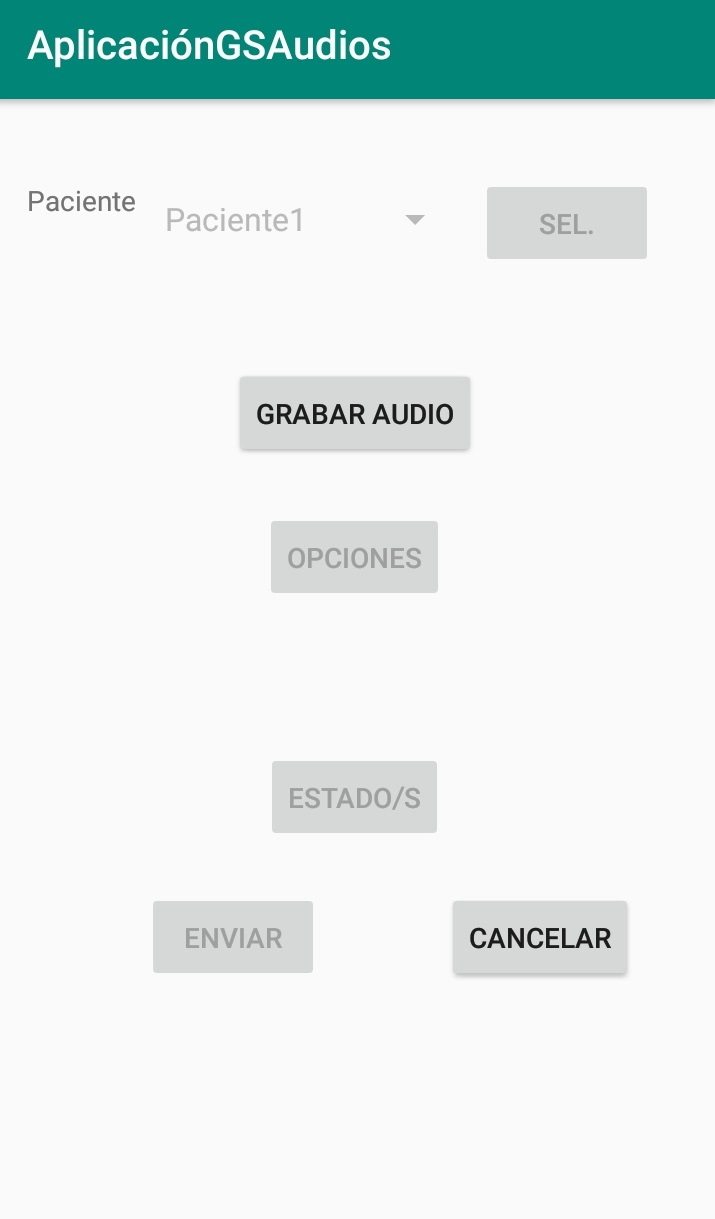
\includegraphics[scale=0.3]{mp2gd}
	\caption{Paciente seleccionado, \textit{Grabar Audio} habilitado.}
	\label{fig:mp2gd}
\end{figure}

Cuando pulsamos el botón \textit{Grabar Audio} se abrirá una nueva pantalla donde podremos grabar el audio correspondiente, como se puede ver en la figura~\ref{gagd}.

\begin{figure}[H]
	\centering
	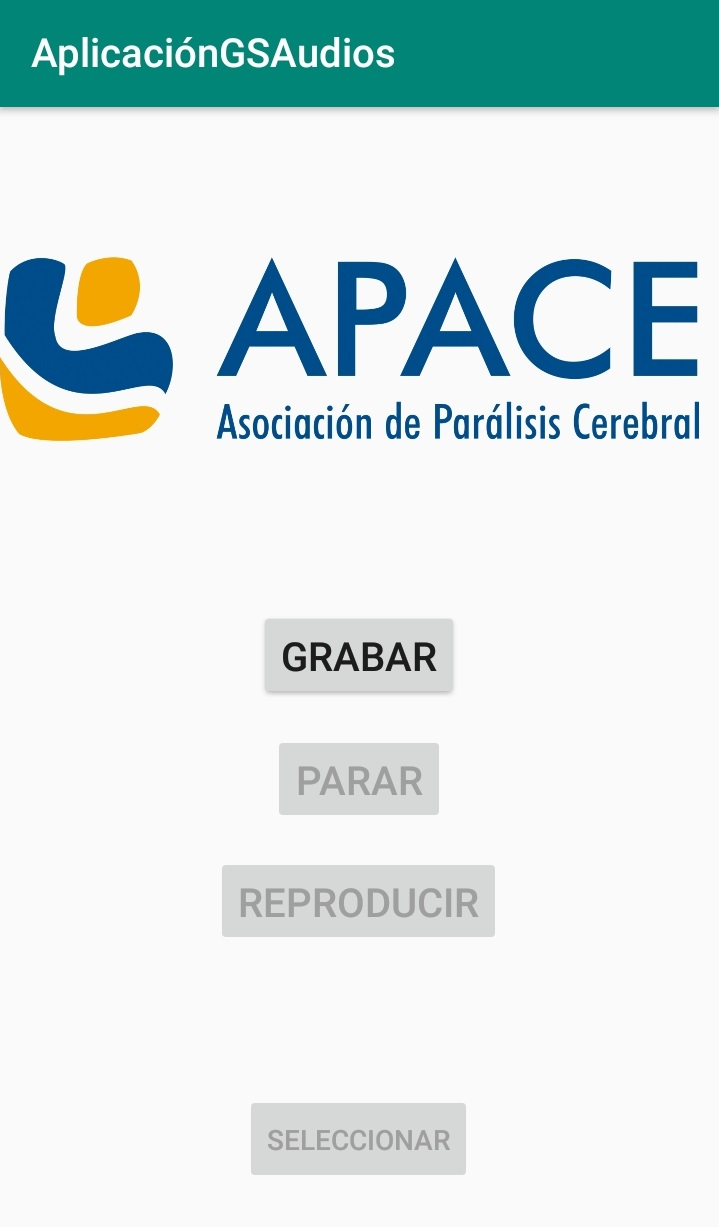
\includegraphics[scale=0.3]{gagd}
	\caption{Pantalla de Grabación de Audios.}
	\label{fig:gagd}
\end{figure}

Como se puede observar esta pantalla tiene 4 botones, pero nada más abrir la pantalla solo tenemos habilitado el botón de \textit{Grabar} que su función es comenzar a grabar el audio una vez lo pulsemos. Una vez pulsado se deshabilitará (para no poder pulsar \textit{Grabar} dos veces) y se habilitará el botón \textit{Parar}, como se puede ver en la figura~\ref{fig:ga2gd}.

\begin{figure}[H]
	\centering
	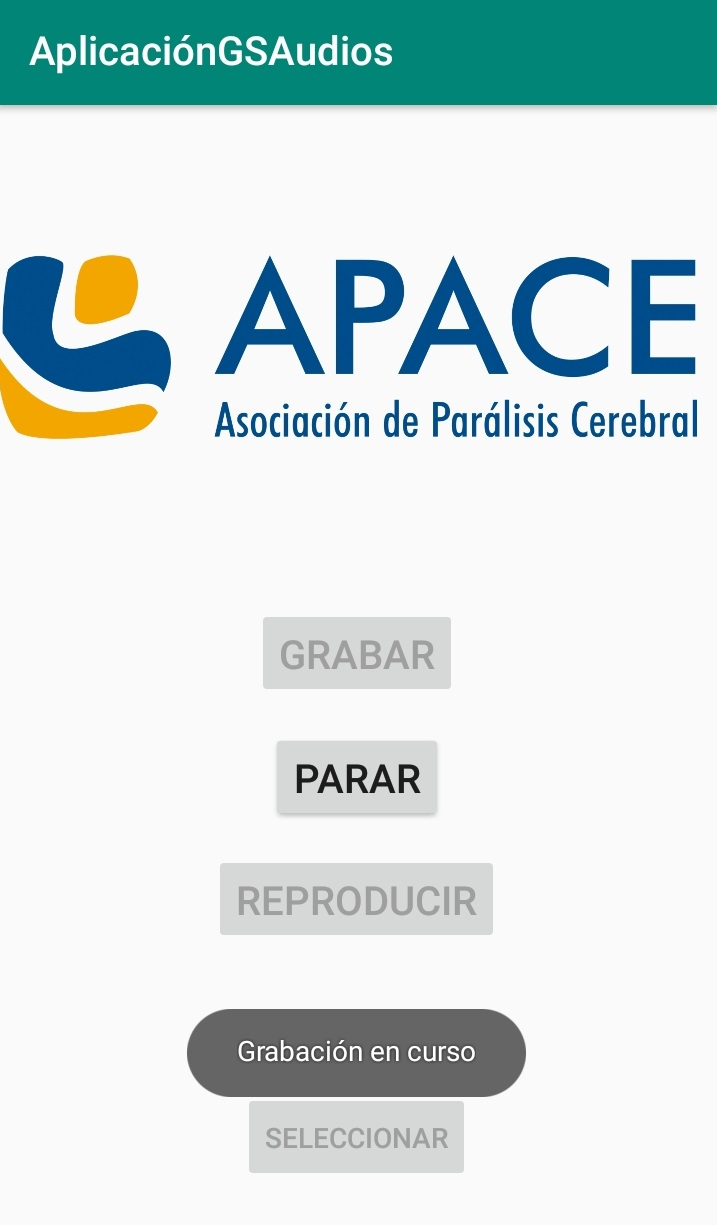
\includegraphics[scale=0.3]{ga2gd}
	\caption{Pulsamos el botón \textit{Grabar}.}
	\label{fig:ga2gd}
\end{figure}

Si pulsamos el botón \textit{Parar} se parará la grabación que habíamos comenzado, además, se habilitarán los botones de \textit{Reproducir} que nos permite reproducir el audio que se acaba de grabar, el botón \textit{Seleccionar} que nos permite seleccionar el audio y volver al menú principal y el botón \textit{Grabar} que nos permite eliminar la grabación actual y comenzar de nuevo una grabación. La interfaz tras pulsar el botón \textit{Parar} se puede ver en la figura~\ref{fig:ga3gd}.

\begin{figure}[H]
	\centering
	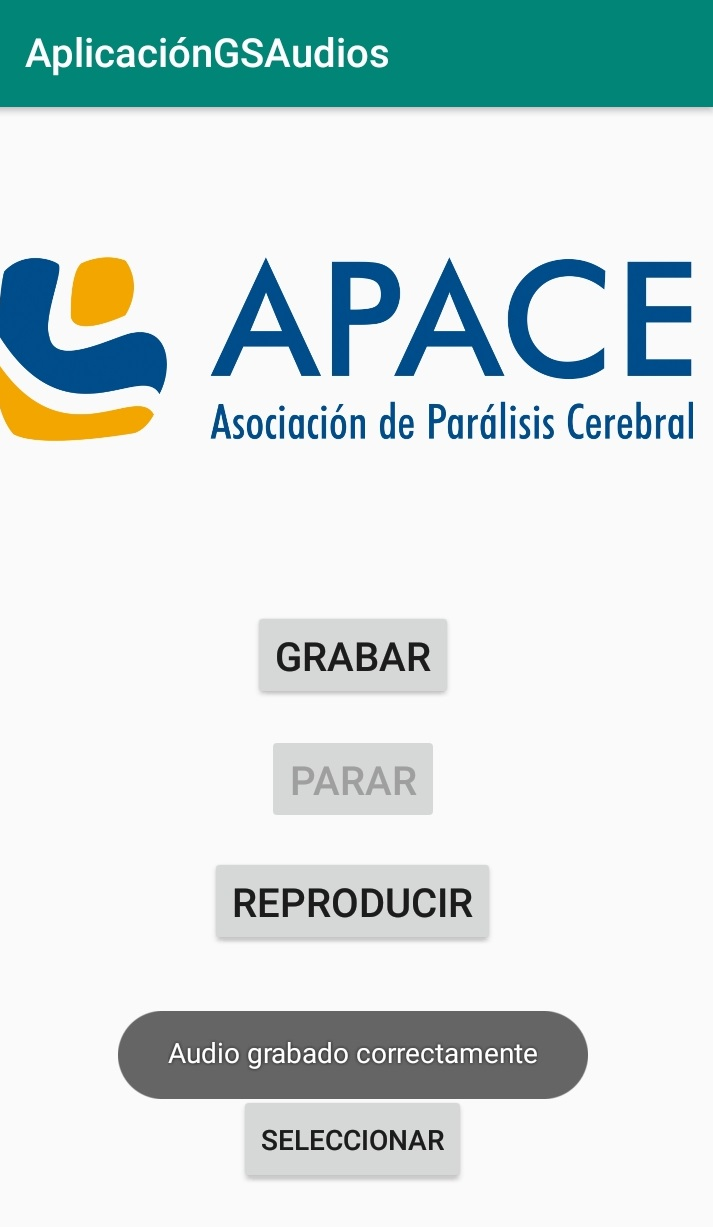
\includegraphics[scale=0.3]{ga3gd}
	\caption{Pulsamos el botón \textit{Parar}.}
	\label{fig:ga3gd}
\end{figure}

Es importante que si se quiere seleccionar el audio se pulse el botón \textit{Seleccionar} tras grabar el audio, ya que si volvemos al menú principal con el botón de ir atrás propio del móvil no se habilitará la siguiente pantalla, la pantalla de las Opciones. El menú principal tras pulsar el botón \textit{Seleccionar} se muestra en la figura~\ref{fig:mp3gd}

\begin{figure}[H]
	\centering
	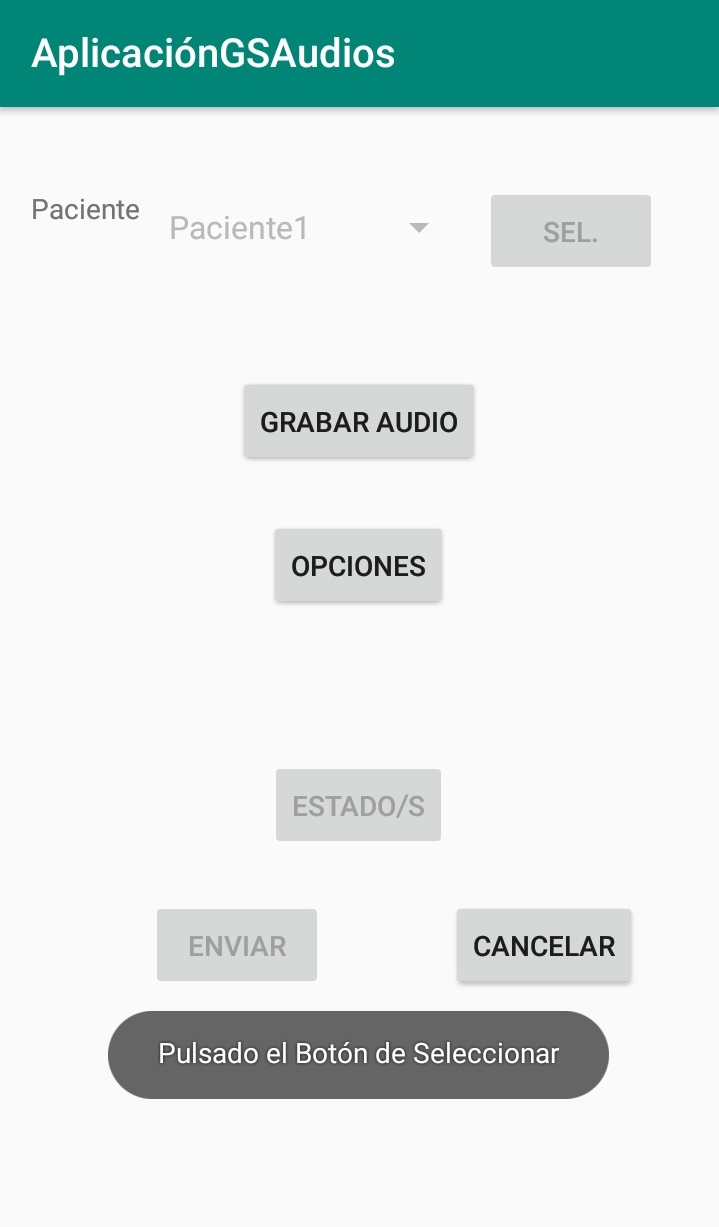
\includegraphics[scale=0.3]{mp3gd}
	\caption{Menú principal tras pulsar el botón \textit{Seleccionar}.}
	\label{fig:mp3gd}
\end{figure}

Como podemos ver, tras pulsar el botón de \textit{Seleccionar} en la pantalla de Grabación de Audio nos dirige hacia la pantalla del menú principal con el botón \textit{Opciones} habilitado, si le pulsamos iremos a la pantalla de Opciones donde podremos seleccionar las opciones adicionales, esta pantalla la podemos ver en la figura~\ref{fig:opgd}.

\begin{figure}[H]
	\centering
	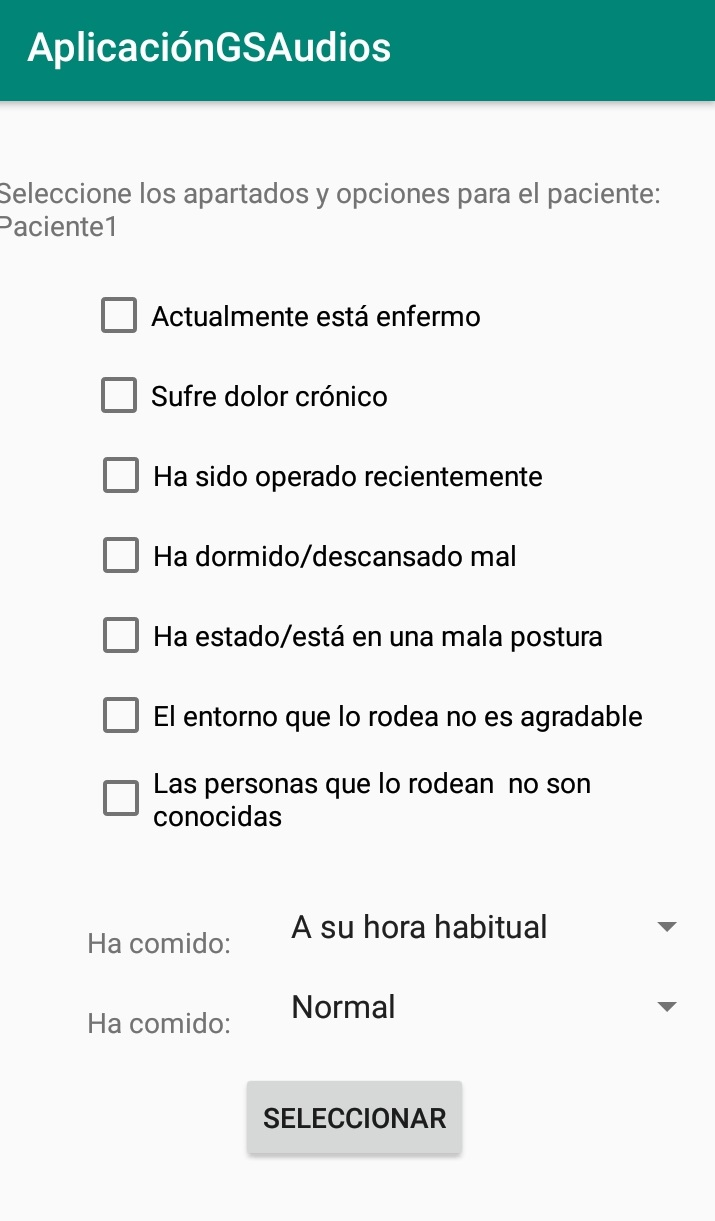
\includegraphics[scale=0.3]{opgd}
	\caption{Pantalla para seleccionar las opciones adicionales.}
	\label{fig:opgd}
\end{figure}

Una vez hayamos rellenado el formulario tenemos que pulsar el botón \textit{Seleccionar} que nos volverá a la pantalla del menú principal. Como pasaba en la pantalla anterior, debemos volver al menú principal a partir de el botón \textit{Seleccionar}, ya que sino no se desbloqueará el botón de \textit{Estado} en el menú principal. El menú principal tras pulsar el botón \textit{Seleccionar} en la pantalla de las opciones se puede ver en la figura~\ref{fig:mp4gd}.

\begin{figure}[H]
	\centering
	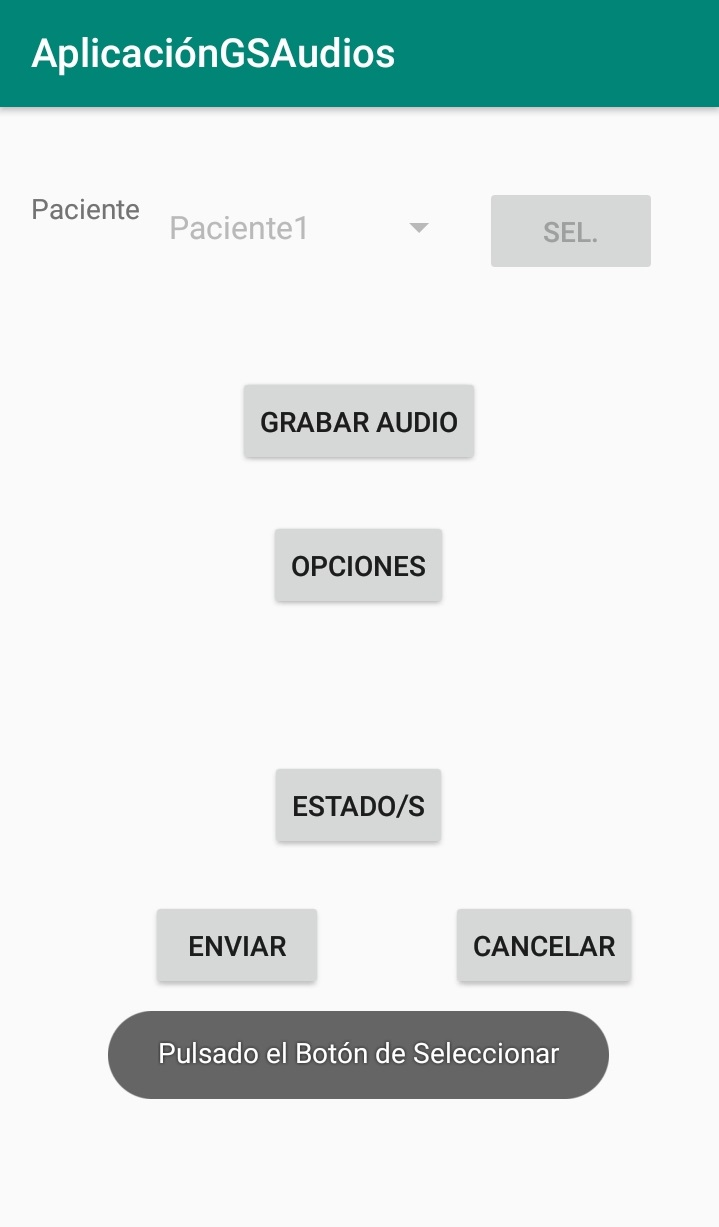
\includegraphics[scale=0.3]{mp4gd}
	\caption{Menú principal tras pulsar el botón \textit{Seleccionar} en la pantalla de opciones.}
	\label{fig:mp4gd}
\end{figure}

Como podemos observar, al pulsar el botón \textit{Seleccionar} en la pantalla de Opciones nos redirige al menú principal con el botón \textit{Estado/s} habilitado. Si pulsamos este botón \textit{Estado/s} nos llevará a la pantalla de selección de estados donde podremos elegir la emoción o respuesta que creemos que tiene el paciente (se puede seleccionar más de uno, pero de distintas columnas, es decir, se puede seleccionar por ejemplo dolor y hambre, pero no se puede seleccionar dolor y sí). Esta pantalla se puede ver en la figura~\ref{ergd}.

\begin{figure}[H]
	\centering
	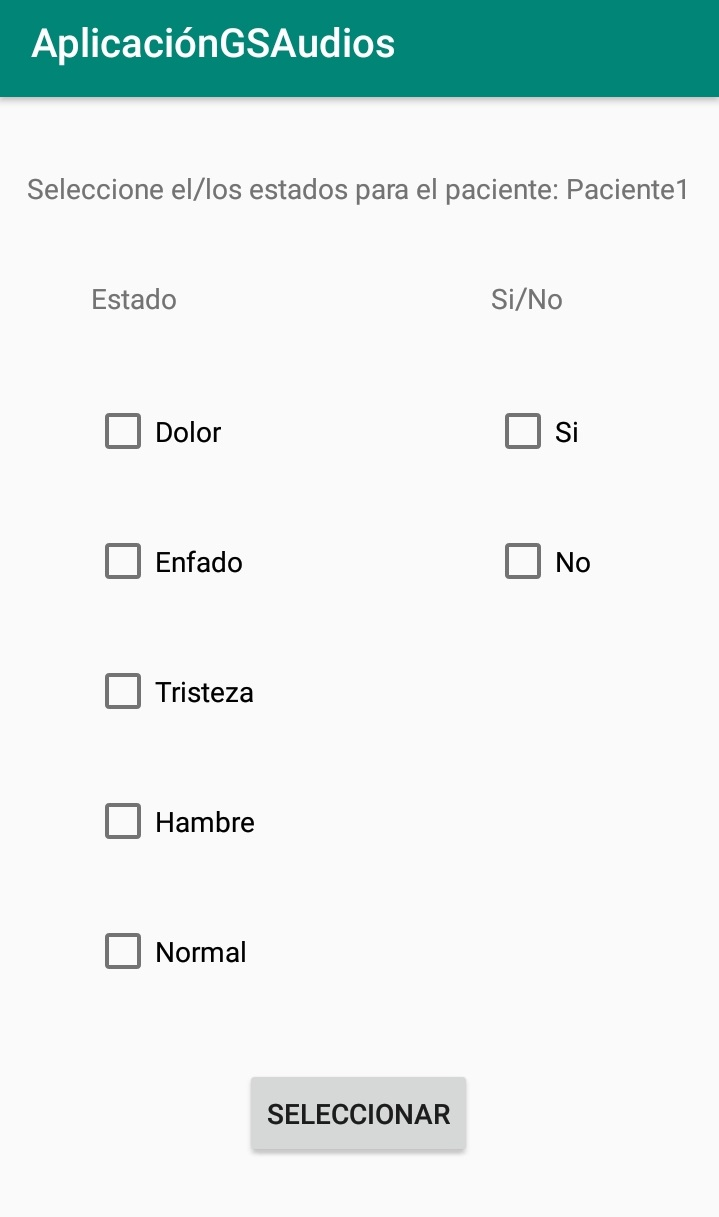
\includegraphics[scale=0.3]{ergd}
	\caption{Pantalla de selección de emociones o respuesta.}
	\label{fig:ergd}
\end{figure}

Como podemos observar en esta pantalla nos permite seleccionar una o más emociones de la primera columna o la respuestas sí o no en la segunda. Con el botón \textit{Seleccionar} guardaremos y volveremos al menú principal, si y solo si hemos cumplido las siguientes reglas en la selección de estados:
\begin{itemize}
	\item Hemos seleccionado elemento/s de solo una de las dos columnas.
	\item Hemos seleccionado algún elemento.
	\item No hemos seleccionado sí y no a la vez.
\end{itemize}

Si no se cumplen todas estas reglas aparecerá un mensaje informativo, y no se nos permitirá volver al menú principal, como se puede ver en la figura~\ref{fig:er2gd}.
\begin{figure}[H]
	\centering
	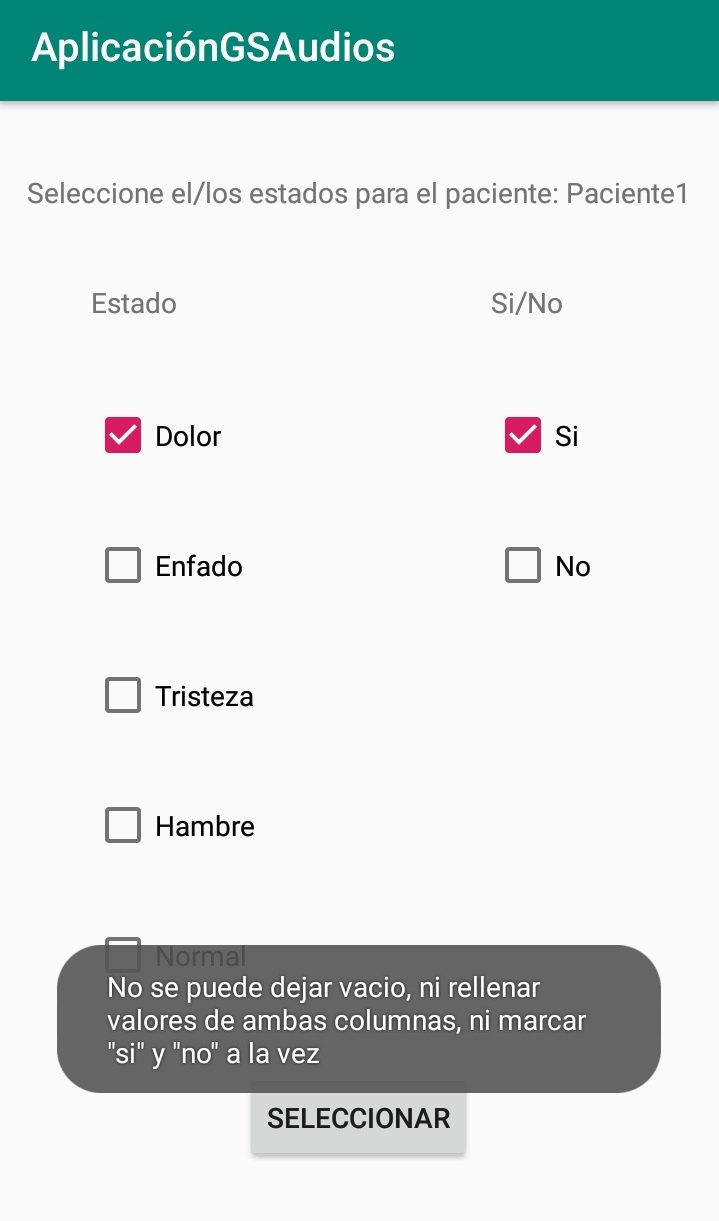
\includegraphics[scale=0.3]{er2gd}
	\caption{Mensaje informativo con el error.}
	\label{fig:er2gd}
\end{figure}
Si por el contrario, no ha ocurrido ningún error al pulsar el botón \textit{Seleccionar} iremos al menú principal teniendo ya todo completado para poder enviar.

Desde el menú principal, tras volver de la pantalla de Estado/s dando al botón \textit{Seleccionar} se nos habrá habilitado el botón de \textit{Enviar} que nos permite comprimir nuestros archivos y enviarlos para la investigación, siempre que haya conexión a Internet, si no tienes conexión a Internet le saldrá el siguiente mensaje (podrá volverse a conectar a Internet y volver a pulsar el botón de \textit{Enviar}), como se puede ver en la figura~\ref{fig:mp5gd}.

\begin{figure}[H]
	\centering
	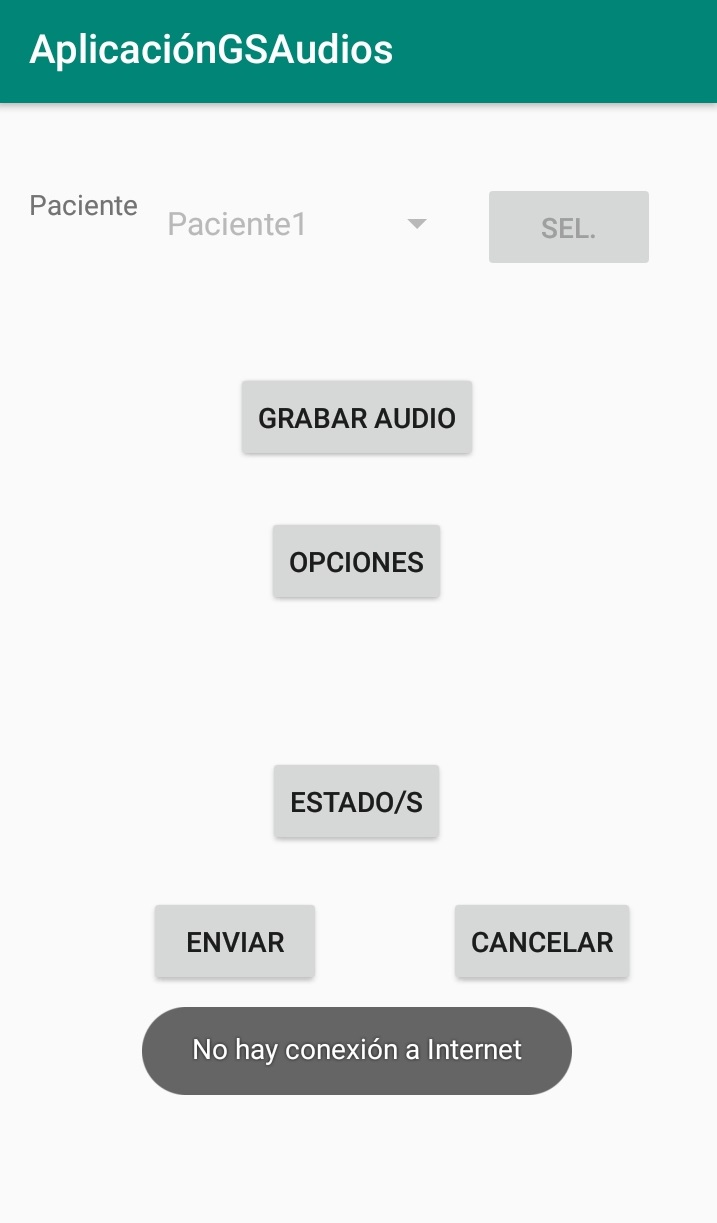
\includegraphics[scale=0.3]{mp5gd}
	\caption{Mensaje de error al intentar enviar sin conexión a Internet.}
	\label{fig:mp5gd}
\end{figure}

Si tenemos conexión el comprimido se generará y se enviará para su posterior investigación.

Cabe destacar que en cualquier momento se puede volver a ir a una pantalla (Grabar Audios, Opciones y Estado/s) una vez visitada, para observar lo que se tiene marcado o para modificarlo.
\section{Aplicación para la interpretación}
\subsection{Uso}
Esta aplicación sirve para interpretar las emociones y las respuestas de las personas con parálisis cerebral de las cuales se han obtenido los datos suficientes como para poder haber creado los algoritmos correspondientes y necesarios. Si el paciente al que desea interpretar no está en la lista de pacientes disponibles ha de seguir grabando datos válidos para ese paciente.
\subsection{Requisitos}
El requisito principal es contar con un dispositivo \textit{smartphone Android} actualizado con una versión \textit{Android} 6.0 o superior y conexión a directa vía \textit{Wi-Fi} al servidor.
\subsubsection{Instalación}
Para poder instalar la aplicación el único requisito que se necesita es conexión a Internet para poder descargarse la aplicación.
\subsubsection{Ejecución}
Para la ejecución de la aplicación se requiere que esta esté instalada, que se acepten los permisos de grabación de audio y de escritura que se preguntan al principio de la ejecución y conexión directa con el servidor.
\subsection{Instalación}
La instalación del prototipo es sencilla, solo hay que descargar el archivo \textit{apk} desde donde se haya sido suministrado (correo, \textit{WhatsApp}, \textit{GitHub}) y realizar los ajustes necesarios para poder descargarla al ser una aplicación ajena a \textit{Play Store}.

Estos ajustes adicionales consisten simplemente aceptar que se descargue esta aplicación exterior a \textit{Play Store}.

Una vez descargada la \textit{apk} la aplicación aparecerá en su menú de aplicaciones instaladas con el nombre de AVC, como se puede ver en la figura~\ref{fig:logoavc}.

\begin{figure}[H]
	\centering
	
\includegraphics[scale=0.6]{logoavc}
	\caption{Logotipo y nombre de la aplicación de interpretación, AVC.}
	\label{fig:logoavc}
\end{figure}

\subsection{Ejecución}
Para la ejecución solo tenemos que seleccionar el logotipo anteriormente mostrado. En la primera ejecución que hagamos del prototipo nos saldrá el siguiente diálogo para pedirnos permisos para poder usar tanto el sistema de grabación de audio como para poder almacenar archivos, debemos dar permisos a ambos pulsando en la opción \textit{Permitir}, es muy importante aceptar estos permisos ya que sino la aplicación se cerrará en la primera vez que queramos grabar un audio. En cualquier caso, si por algún error se ha denegado los permisos y la aplicación se ha cerrado se puede volver a abrir y nos volverá a pedir aceptar los permisos. La forma en la que se piden estos permisos se puede ver en las figuras~\ref{fig:avcper1} y ~\ref{fig:avcper2}.

\begin{figure}[H]
	\centering
	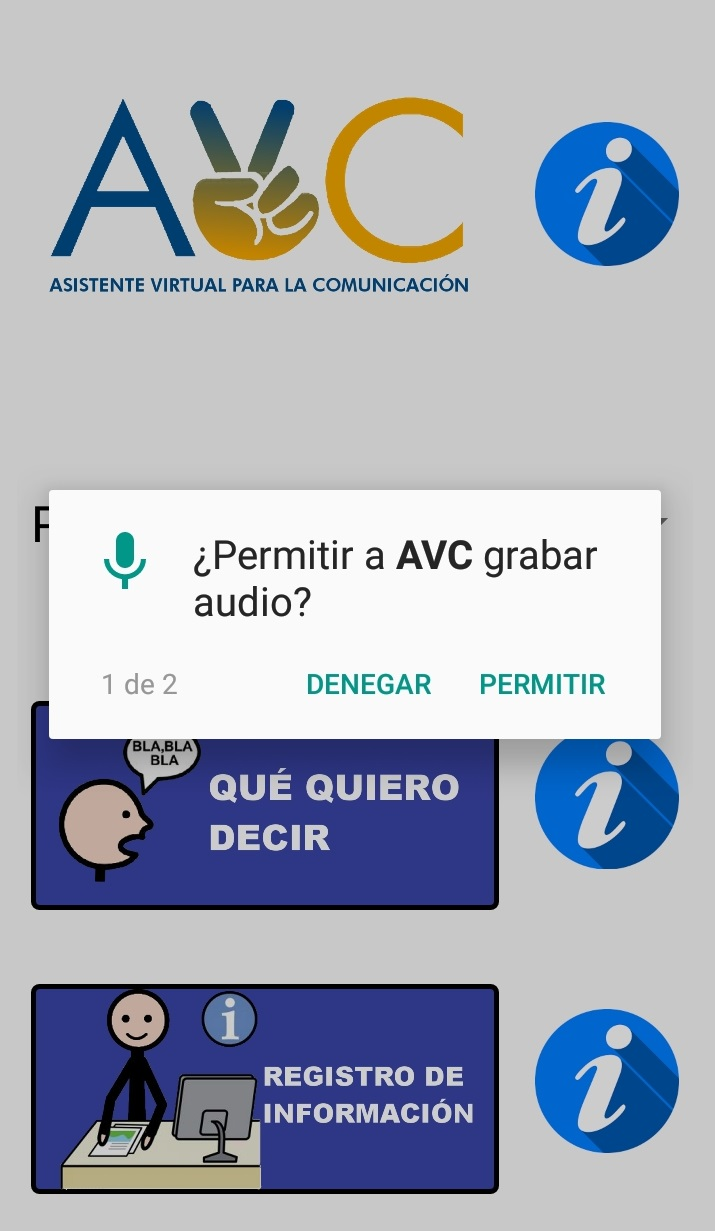
\includegraphics[scale=0.3]{avcper1}
	\caption{Permisos de grabación de audio en AVC.}
	\label{fig:avcper1}
\end{figure}

\begin{figure}[H]
	\centering
	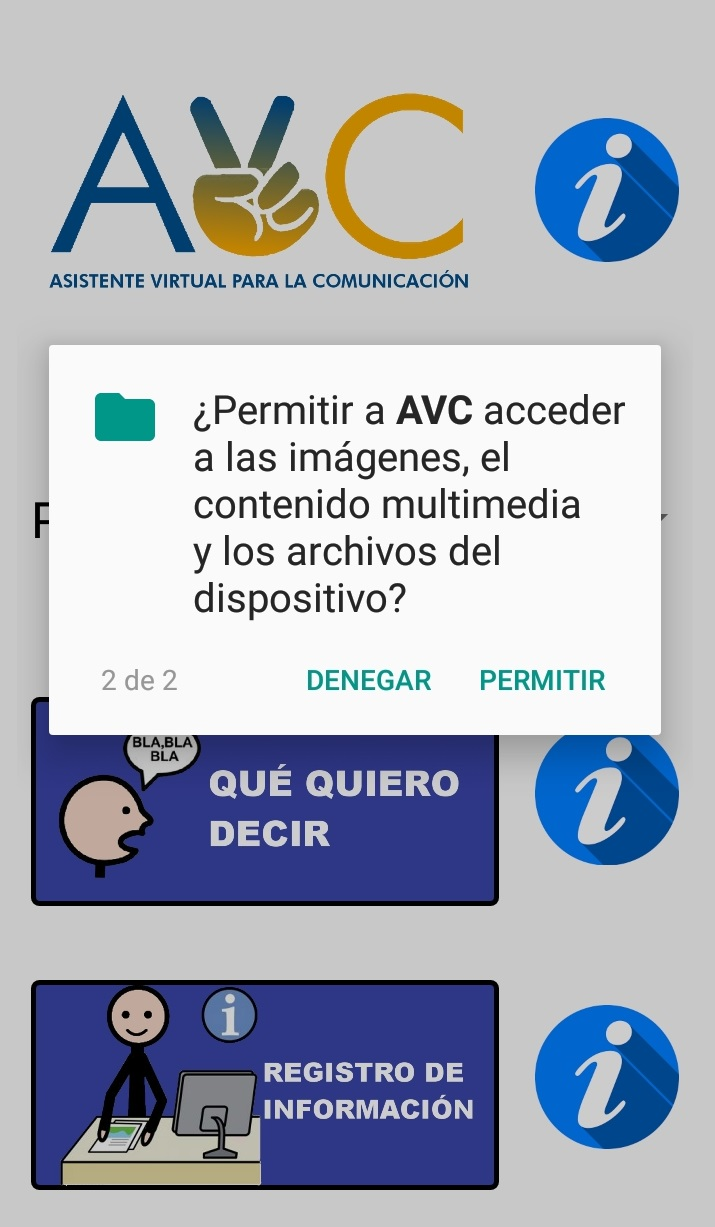
\includegraphics[scale=0.3]{avcper2}
	\caption{Permisos para el acceso a multimedia en AVC.}
	\label{fig:avcper2}
\end{figure}

Después de aceptar los permisos tendremos acceso al menú principal de la aplicación, aquí podremos seleccionar el paciente con el cual queremos trabajar (el último paciente que se seleccionó antes de cerrar la aplicación será el paciente que aparezca como seleccionado cuando volvamos a ejecutar la aplicación). El menú principal de la aplicación se puede ver en la figura~\ref{mpavc}.

\begin{figure}[H]
	\centering
	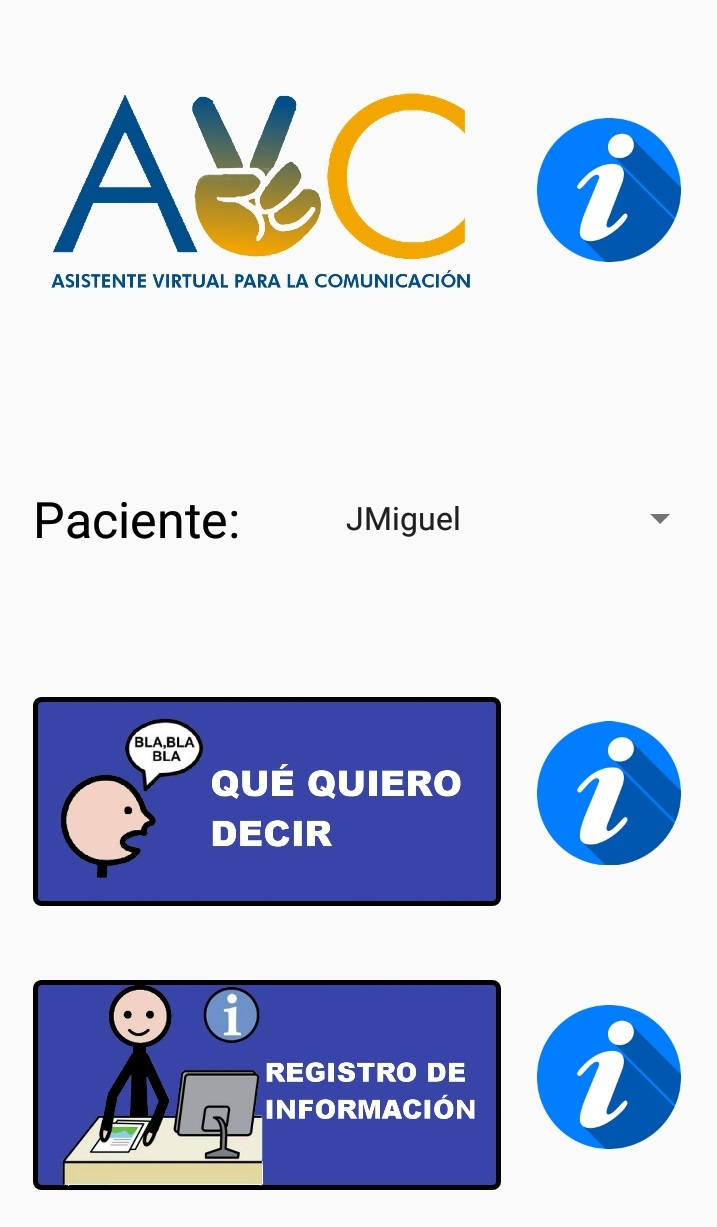
\includegraphics[scale=0.3]{mpavc}
	\caption{Menú principal de la aplicación AVC.}
	\label{fig:mpavc}
\end{figure}

Tras haber seleccionado a nuestro paciente podemos hacer dos cosas diferentes, o podemos modificar las opciones adicionales relacionadas con ese paciente o podemos interpretar una emoción o una respuesta.

Si queremos modificar o ver las opciones adicionales del paciente seleccionado tenemos que pulsar el botón de \textit{Registro de Información}, que nos llevará a la pantalla donde podremos ver las opciones guardadas para ese paciente, como se puede ver en la figura~\ref{fig:opcavc}.

\begin{figure}[H]
	\centering
	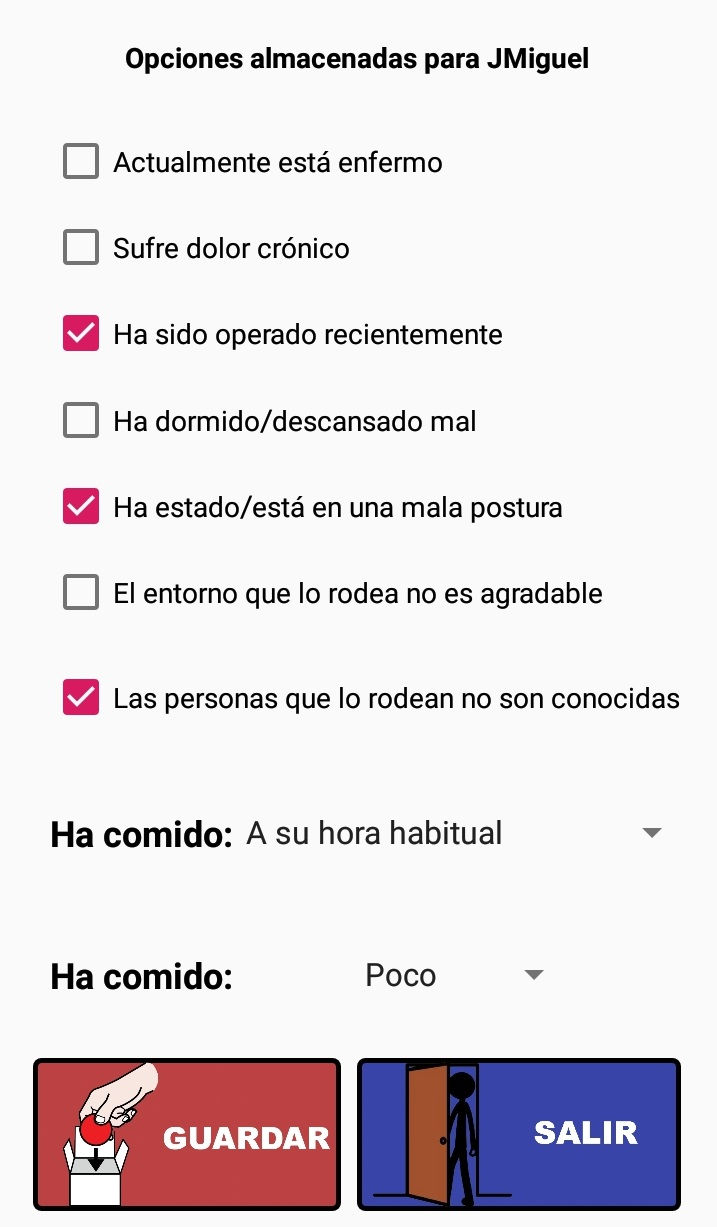
\includegraphics[scale=0.3]{opcavc}
	\caption{Pantalla con las opciones cargadas del paciente seleccionado.}
	\label{fig:opcavc}
\end{figure}

Al cargar la pantalla se verán las opciones almacenadas para el paciente seleccionado, aquí podemos salir si no queremos modificar ninguna opción pulsando el botón \textit{Salir} o podemos modificar alguna de las opciones, entonces el botón \textit{Guardar} se pondrá en azul por lo que estaría disponible, y pulsándolo haría que se guarden las opciones. El cambio en el botón \textit{Guardar} se puede observar en la siguiente figura~\ref{fig:opc2avc}.

\begin{figure}[H]
	\centering
	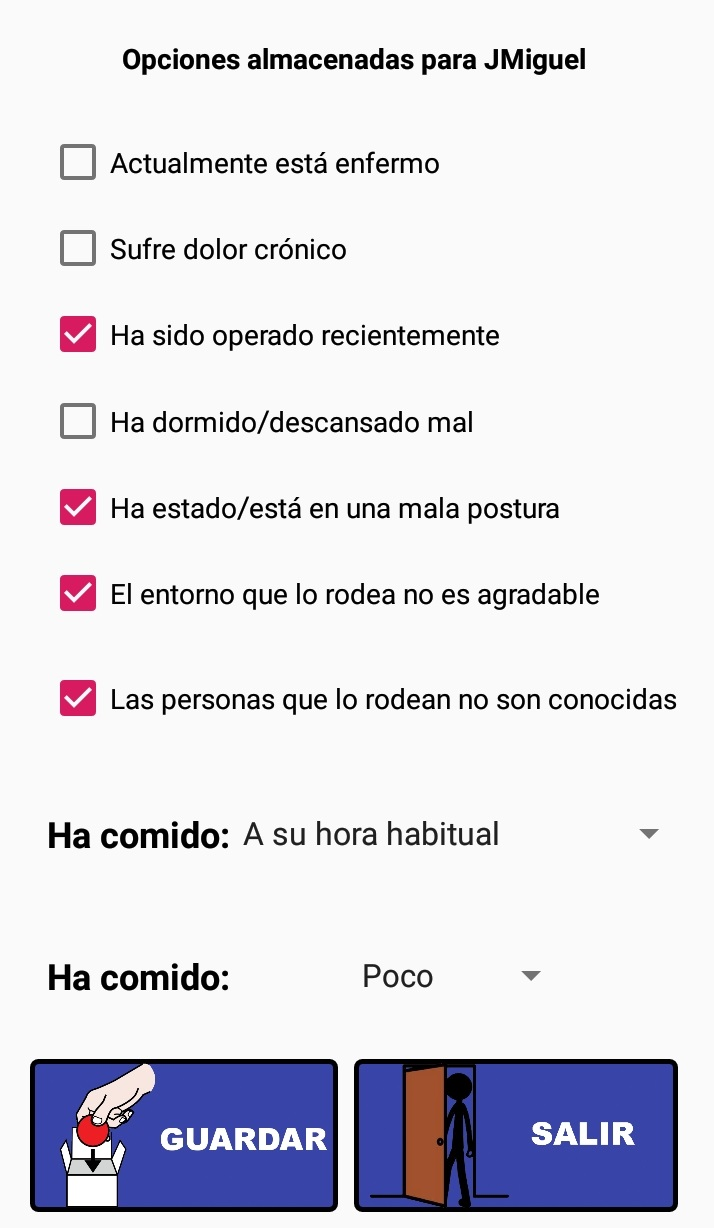
\includegraphics[scale=0.3]{opc2avc}
	\caption{Botón \textit{Guardar} habilitado.}
	\label{fig:opc2avc}
\end{figure}

Una vez pulsados el botón \textit{Salir} o \textit{Guardar} volveremos a la pantalla principal.

Si por el contrario lo que queremos es interpretar una emoción o una respuesta tenemos que pulsar en el menú principal \textit{Qué quiero decir}, este nos llevará a una nueva pantalla, la pantalla de selección de interpretación, que se puede ver en la figura~\ref{fig:interpavc}.

\begin{figure}[H]
	\centering
	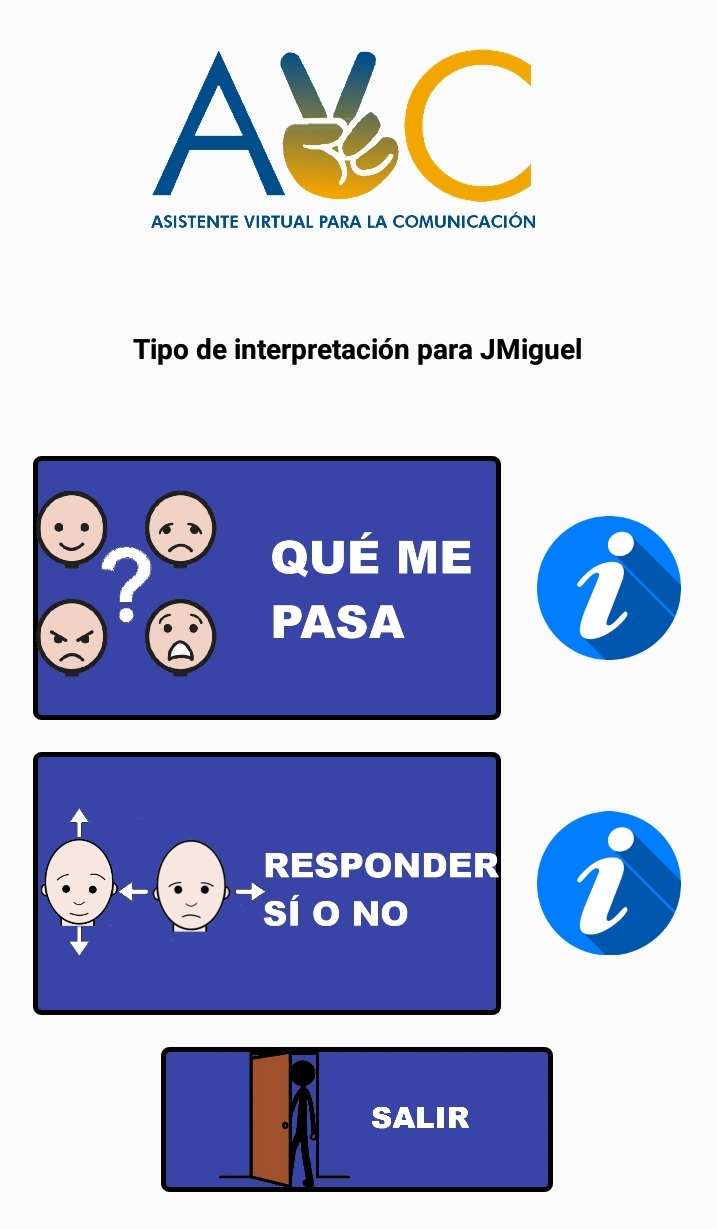
\includegraphics[scale=0.3]{interpavc}
	\caption{Pantalla de selección del tipo de interpretación.}
	\label{fig:interpavc}
\end{figure}

En esta pantalla podemos pulsar el botón \textit{Salir} que nos llevaría de nuevo al menú principal, o podemos pulsar en los botones de \textit{Qué me pasa} si queremos interpretar una emoción, o \textit{Responder sí o no} si queremos interpretar una respuesta.

Cualquier tipo de interpretación que pulsemos nos llevará a la pantalla de grabación del audio, que se puede ver en la figura~\ref{fig:gaavc}.

\begin{figure}[H]
	\centering
	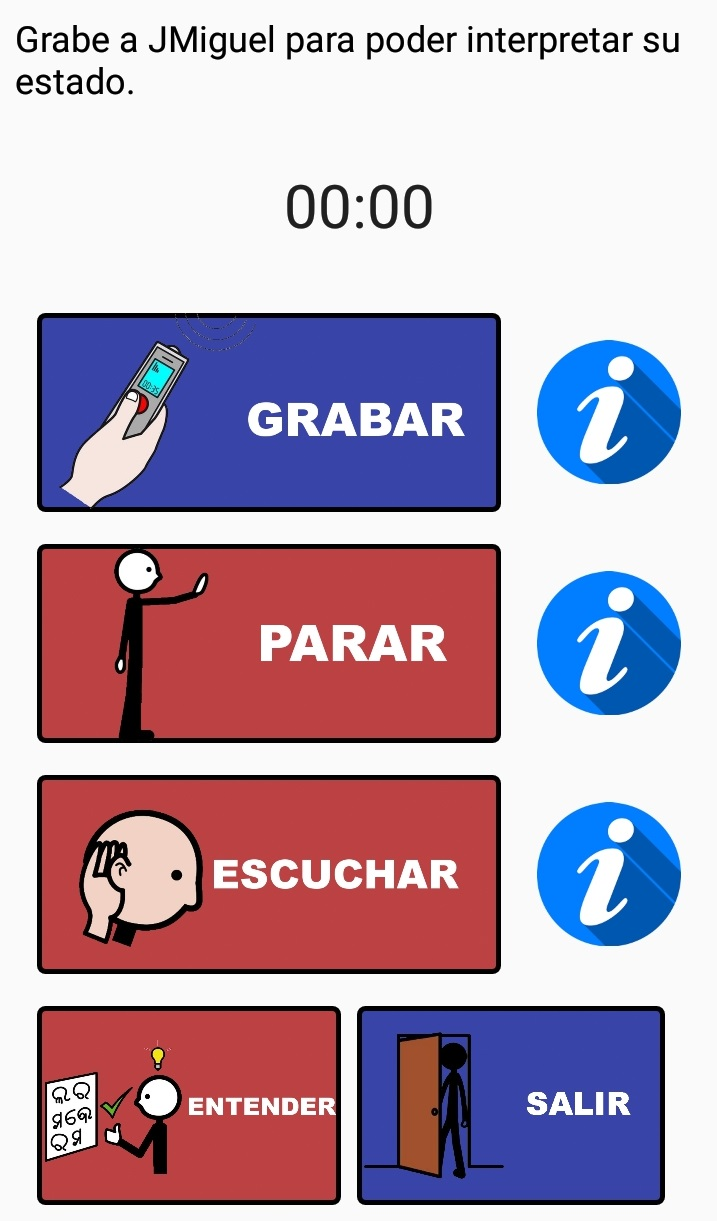
\includegraphics[scale=0.3]{gaavc}
	\caption{Pantalla de grabación del audio.}
	\label{fig:gaavc}
\end{figure}

En esta pantalla podemos grabar el audio que queremos interpretar. Como en el resto de las pantallas, tenemos el botón \textit{Salir} que nos devuelve a la pantalla anterior, la pantalla de selección de interpretación.

Si por el contrario queremos grabar un audio solo tenemos que pulsar el botón \textit{Grabar} para comenzar a grabar, entonces el contador empezará a sumar mostrándonos el tiempo de grabación, como se puede ver en la figura~\ref{fig:ga2avc}.

\begin{figure}[H]
	\centering
	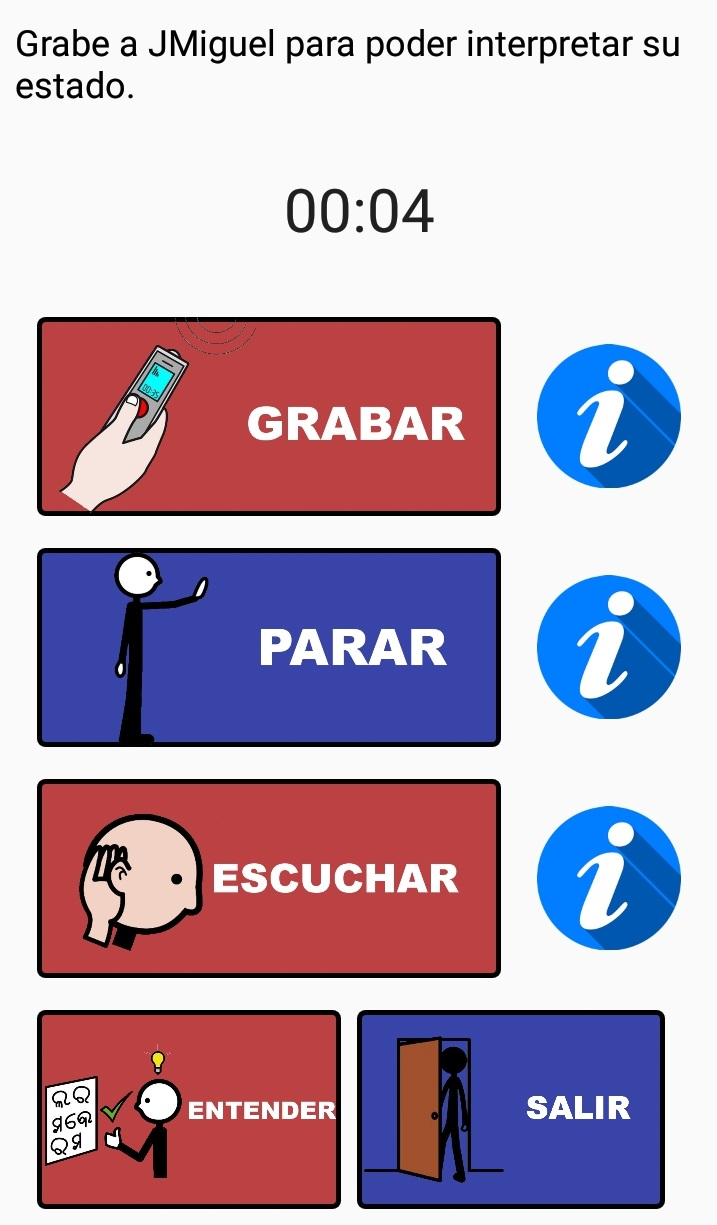
\includegraphics[scale=0.3]{ga2avc}
	\caption{Empezamos a grabar, tras pulsar \textit{Grabar}.}
	\label{fig:ga2avc}
\end{figure}

Si queremos parar de grabar entonces tenemos que pulsar el botón \textit{Parar}, entonces el audio se guardará y podremos escucharlo pulsando el botón \textit{Escuchar} o intepretarlo pulsando el botón \textit{Entender}, como se puede ver en la figura~\ref{fig:ga3avc}.

\begin{figure}[H]
	\centering
	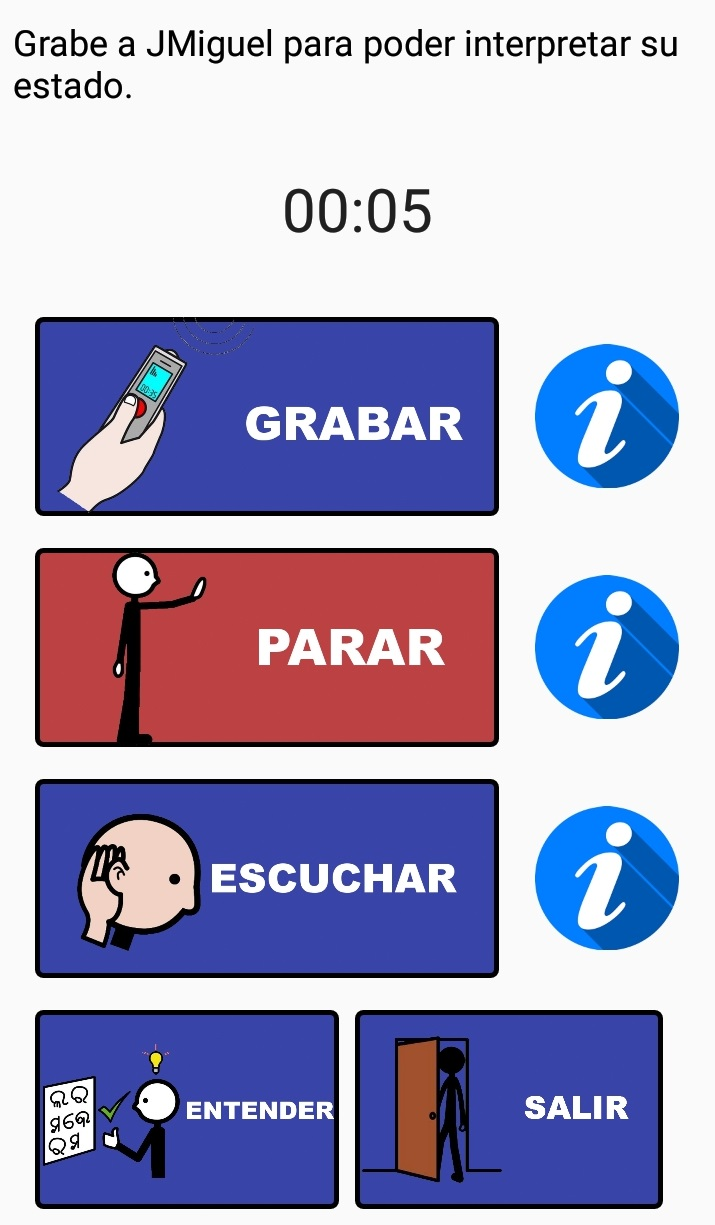
\includegraphics[scale=0.3]{ga3avc}
	\caption{Paramos la grabación, tras pulsar \textit{Parar}.}
	\label{fig:ga3avc}
\end{figure}

Una vez grabado el audio podemos volver a grabarlo pulsando de nuevo el botón \textit{Grabar}, que iniciaría de nuevo la grabación. Si por el contrario el audio es correcto y es el que queremos interpretar tenemos que pulsar en el botón \textit{Entender} que nos llevará a la pantalla donde encontraremos el resultado de la interpretación. Un ejemplo de un resultado de una interpretación se puede ver en la figura~\ref{fig:resavc}.

\begin{figure}[H]
	\centering
	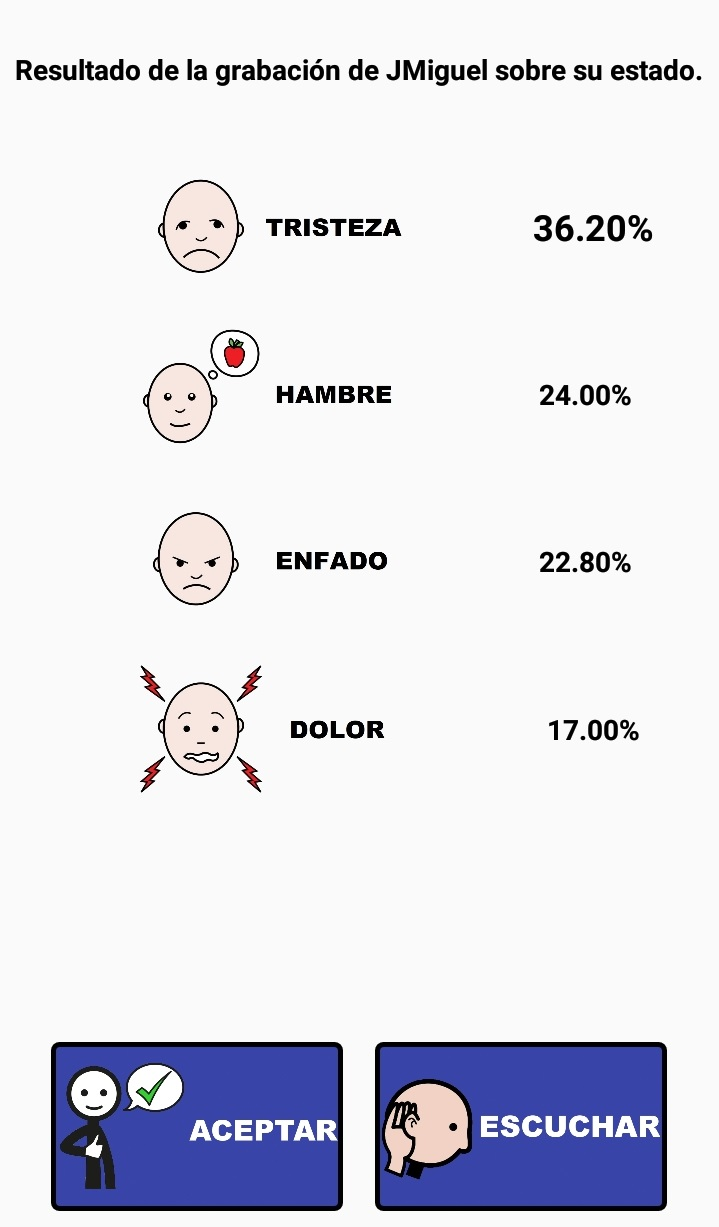
\includegraphics[scale=0.3]{resavc}
	\caption{Ejemplo de la pantalla con el resultado de una interpretación.}
	\label{fig:resavc}
\end{figure}

En esta pantalla podremos ver el resultado con porcentajes de la interpretación, siendo el que viene más arriba el resultado con mayor porcentaje. En esta pantalla podemos volver a escuchar el audio que hemos interpretado pulsando el botón \textit{Escuchar}, o podemos salir al menú principal pulsando el botón \textit{Aceptar}.

Además, a lo largo de la aplicación nos podemos encontrar con distintos botones de información a la derecha de otros botones, estos botones de información nos abren un dialogo en el cual se nos comunica vía texto en lectura fácil y por audio lo que hace el botón que tiene a la izquierda, un ejemplo de estos diálogos se puede ver en la figura~\ref{fig:diaavc}.

\begin{figure}[H]
	\centering
	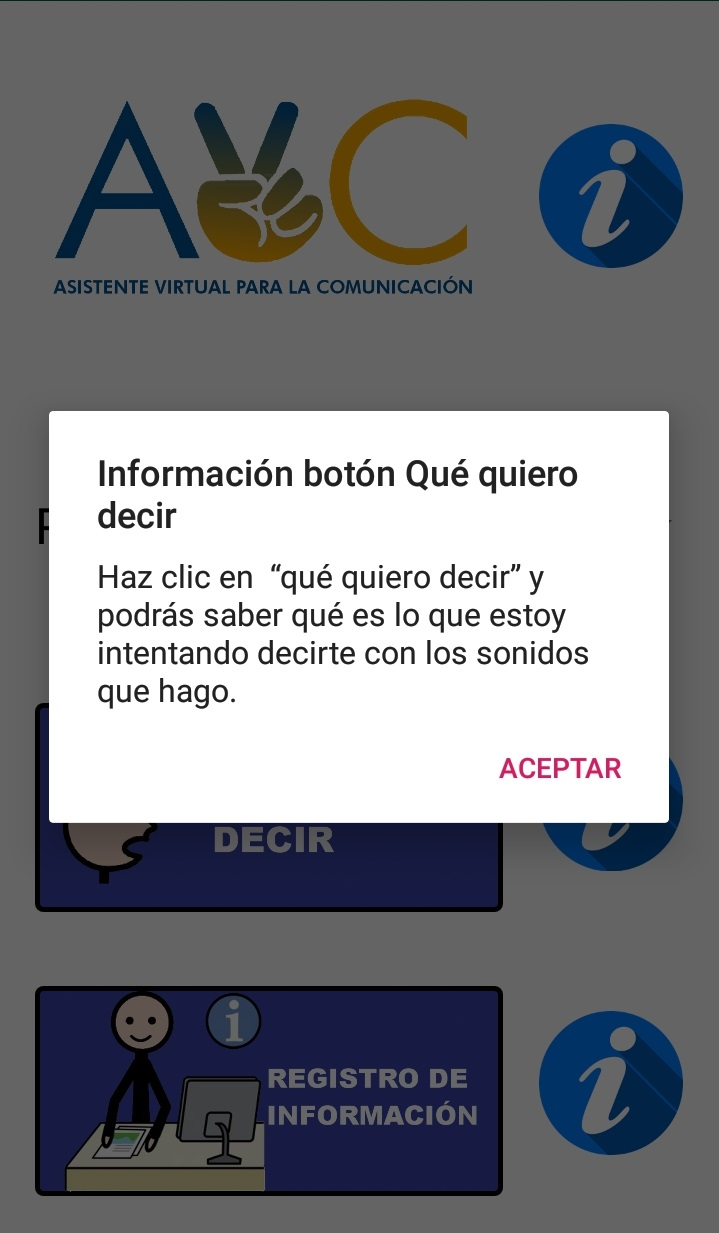
\includegraphics[scale=0.3]{dialogo}
	\caption{Ejemplo de diálogo informativo.}
	\label{fig:diaavc}
\end{figure}


\bibliographystyle{plain}
\bibliography{bibliografiaAnexos}

\end{document}
